\chapter{The Climatica Application}\label{APP}

This chapter describes the design and implementation of Climatica.
Section~\ref{APP_REQ} derives the requirements from the project context.
Section~\ref{APP_ARCH} presents the architecture and key design decisions,
including the migration from a React SPA to a Next.js full-stack application.
Section~\ref{APP_TECH} justifies the technology choices made during development.
Section~\ref{APP_QA} describes the quality assurance strategy.
Section~\ref{APP_PROTO} walks through the four implemented pages.

% * ─── 3.1 Requirements ─────────────────────────────────────────────────────────
\section{Requirements}\label{APP_REQ}

\subsection{Project Context and Elicitation}\label{APP_REQ_CONTEXT}

Climatica was initiated as a Bachelor's thesis internship project at the
Universidad de Valladolid. The starting point was minimal: the supervision team
provided access to the WorldClim Virtual Semantic API (SCRAPI), its 16-page
documentation, and a reference to ClimateCharts.net as an example of the kind
of tool that could be built on top of such data. No formal requirements document
was produced; instead, the scope was agreed iteratively through fortnightly
meetings with the supervision team.

The first weeks of the project were devoted to understanding the underlying
technologies --- RDF, SPARQL, the WorldClim data model --- and building a minimal
prototype (Figure~\ref{fig:proto_v1}) to validate the API integration. This early
version featured a single page with a city search field, a Leaflet map, and a
standard climograph with filters displayed as a collapsible panel below the
search bar. Based on feedback from this prototype, the design was progressively
refined into the four-page application described in Section~\ref{APP_PROTO}.

\begin{figure}[t]
  \centering
  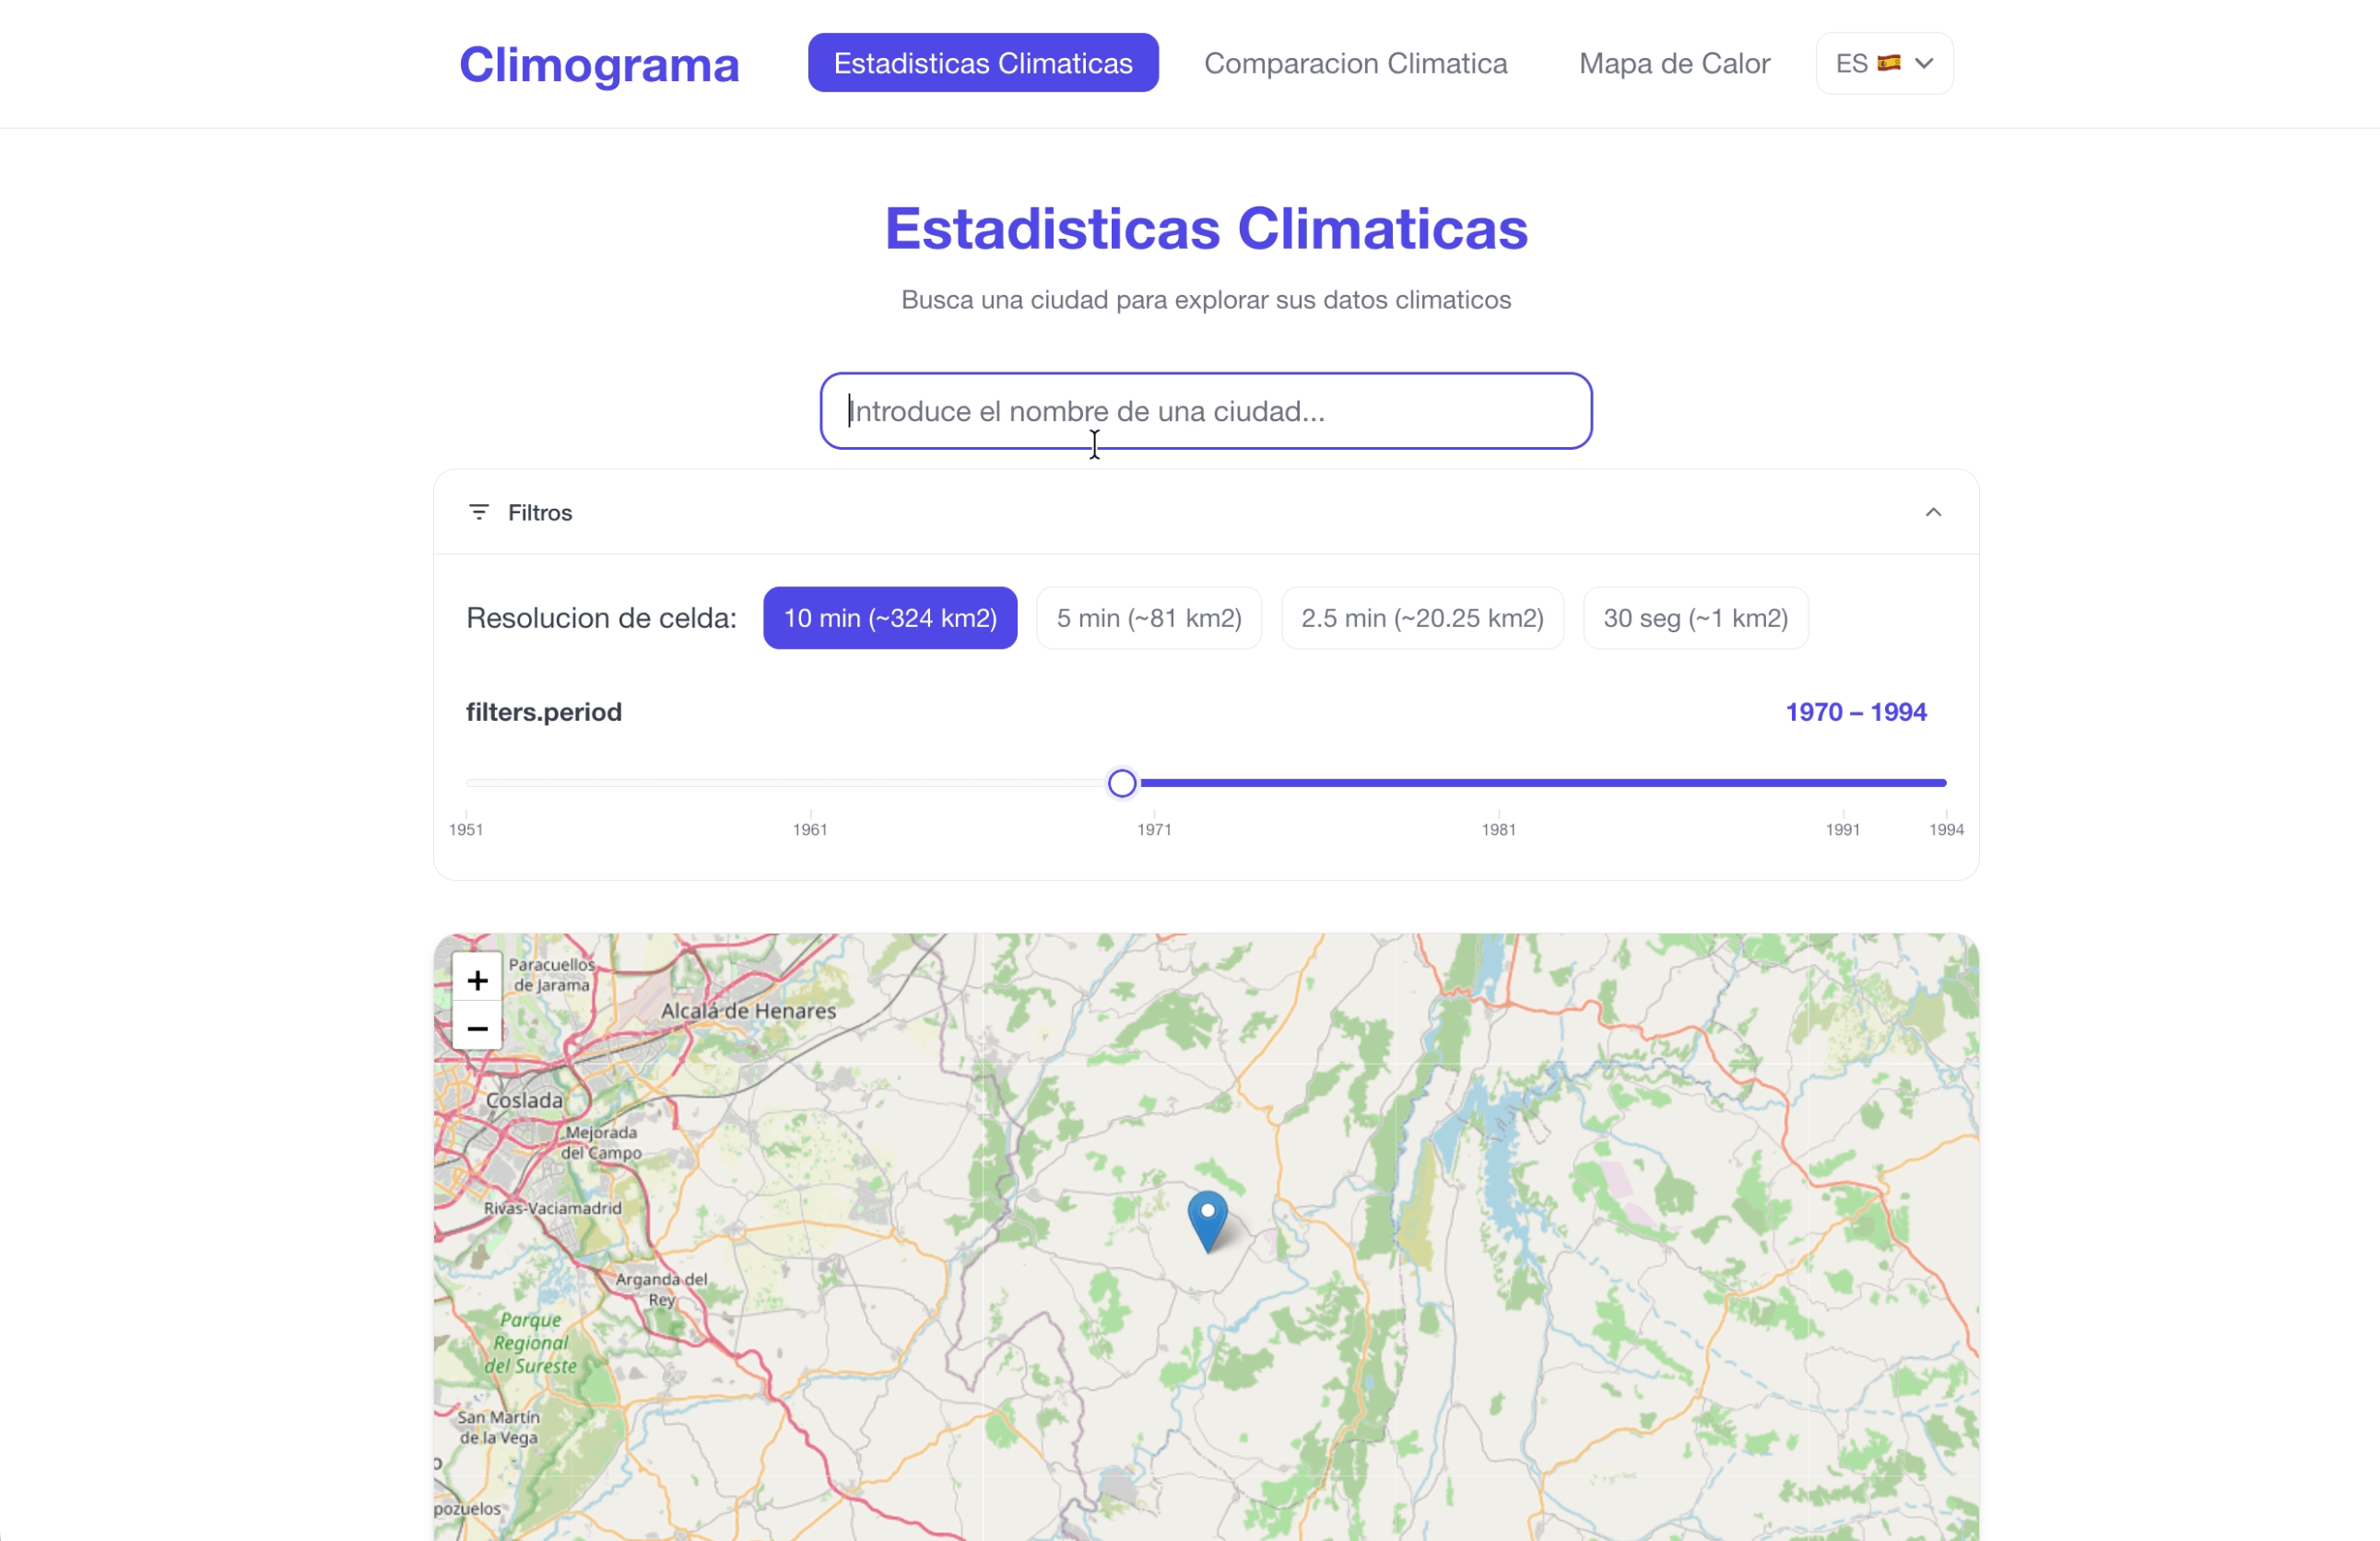
\includegraphics[width=0.9\textwidth]{Images/climatica-v1.png}
  \caption{Early prototype of Climatica (first iteration). The filter panel
    expanded below the search bar; the single page combined map, chart, and
    controls without a persistent sidebar. This layout was later reorganised
    into a fixed sidebar and four separate pages.}
  \label{fig:proto_v1}
\end{figure}

\subsection{Functional Requirements}\label{APP_REQ_FUNC}

The following functional requirements were established through the iterative
process described in Section~\ref{INTRO_MET}. Requirements marked with an
asterisk (*) emerged during later review meetings rather than at the outset.

\begin{enumerate}
  \item \textbf{FR1 --- Location search.} The user shall be able to type the
    name of any populated place worldwide --- including cities, towns, and
    villages --- and select from a ranked list of matching results covering
    the entire globe.

  \item \textbf{FR2 --- Location by coordinates.} The user shall be able to
    enter a latitude/longitude pair directly in the search bar to retrieve
    climate data for any arbitrary point.

  \item \textbf{FR3 --- Location by map click.} The user shall be able to click
    any point on the interactive map to retrieve climate data for that location.

  \item \textbf{FR4 --- Use my location.} The user shall be able to use the
    browser's geolocation API to centre the map and retrieve climate data for
    their current position.

  \item \textbf{FR5 --- City climate profile.} For a selected city, the
    application shall display monthly minimum temperature, maximum temperature,
    average temperature, and precipitation, together with summary statistics
    (annual mean temperature, total precipitation, altitude, number of arid
    months).

  \item \textbf{FR6 --- Standard climogram.} The city climate profile shall be
    available as a standard bar-and-line chart showing precipitation bars and
    temperature lines.

  \item \textbf{FR7 --- Walter-Lieth climatogram.*} The city climate profile
    shall also be available as a Walter-Lieth diagram with correct arid/humid
    area shading.

  \item \textbf{FR8 --- City comparison.*} The user shall be able to select two
    cities and view their climate profiles side by side on shared axes, together
    with summary statistics and derived insights (warmer city, more rainfall,
    hottest month, coldest month).

  \item \textbf{FR9 --- Period comparison.*} The user shall be able to select
    one city and compare its climate across two to five time references ---
    either two 30-year climate normals or up to five individual weather years
    --- with trend indicators showing the direction and magnitude of change.

  \item \textbf{FR10 --- Regional heatmap.} The user shall be able to draw a
    bounding box or freeform polygon on the map and view a spatially resolved
    heatmap of any climate variable for any selected month.

  \item \textbf{FR11 --- Filter controls.} The user shall be able to filter all
    views by dataset (Climate / Weather), time period or year, climate variables,
    grid resolution, and month, with invalid combinations automatically disabled.

  \item \textbf{FR12 --- Data export.} The user shall be able to export chart
    data as CSV and as a PNG image.

  \item \textbf{FR13 --- Internationalisation.} The interface shall be available
    in English, Spanish, and Ukrainian, with city names displayed in the active
    language.
\end{enumerate}

\subsection{Non-Functional Requirements}\label{APP_REQ_NONFUNC}

\begin{enumerate}
  \item \textbf{NFR1 --- No registration.} The application shall be usable
    without creating an account.

  \item \textbf{NFR2 --- Secure API key handling.} The WorldClim Bearer token
    shall never be exposed to the browser; all SCRAPI calls shall be proxied
    through a server-side route handler.

  \item \textbf{NFR3 --- Shareable state.} Bounding box coordinates, city
    selections, and period selections shall be reflected in URL search parameters
    so that a specific view can be shared by copying the URL.

  \item \textbf{NFR4 --- Persistent preferences.} The user's last selected city,
    comparison cities, filter settings, and language preference shall survive a
    page reload.

  \item \textbf{NFR5 --- Type safety.} All API responses, domain data shapes,
    and component props shall be fully typed in TypeScript; no \texttt{any}
    types in production code.

  \item \textbf{NFR6 --- Code quality gate.} Every commit shall pass a
    Continuous Integration (CI) check comprising TypeScript compilation,
    ESLint, and Prettier format verification, followed by a separate pipeline
    that runs the full unit and end-to-end test suites.
\end{enumerate}


% * ─── 3.2 Architecture ─────────────────────────────────────────────────────────
\section{Architecture}\label{APP_ARCH}

\subsection{Evolution of the Architecture}\label{APP_ARCH_EVOLUTION}

Climatica was originally built as a pure React~\cite{react} single-page
application (SPA)~\cite{flanagan2020spa} bundled with Vite~\cite{vite} and
deployed as a static file set. In this version, all external API calls --- to
SCRAPI and Wikidata --- were issued directly from the browser. City search
relied on a two-step Wikidata pipeline: a \texttt{wbsearchentities} call
retrieved up to 100 candidate entities matching the user's query, which were
then filtered by a SPARQL query to retain only instances of human settlement
(\texttt{wdt:P31/wdt:P279* wd:Q486972}), ranked by a popularity score derived
from sitelink count and statement count, and capped at ten results.

This approach proved adequate for a prototype but introduced two significant
limitations as the application matured. First, Wikidata applies soft-throttling
to high-frequency queries from a single origin: under interactive typing, the
search bar could exhaust the allowed request rate, causing intermittent failures
with no clean recovery path. Second, the Wikidata pipeline offered limited
control over result ranking; surfacing the most relevant city for a given query
required heuristics built on top of a remote API that could not be tuned or
extended without changing the query logic.

To address both issues, the architecture was redesigned around Next.js~16~\cite{nextjs}
with the App Router. The key changes were: (1)~replacing the Wikidata city-search
pipeline with a locally hosted Apache Solr index, giving full control over
ranking, tokenisation, and query performance; (2)~introducing server-side route
handlers that proxy all SCRAPI and Solr requests, keeping the WorldClim Bearer
token off the client; and (3)~adding a Redis caching layer in front of both
Solr and SCRAPI to reduce latency for repeated queries.

Table~\ref{tab:arch_comparison} summarises the key differences between the two
versions.

\begin{table}[H]
  \centering
  \caption{Architecture comparison: React SPA (v1) vs.\ Next.js full-stack (v2).}
  \label{tab:arch_comparison}
  \small
  \begin{tabular}{p{3.2cm}p{4.8cm}p{4.8cm}}
    \toprule
    \textbf{Aspect} & \textbf{React SPA (v1)} & \textbf{Next.js (v2)} \\
    \midrule
    Framework       & React~18 + Vite        & Next.js~16 (App Router) \\
    City search     & Wikidata SPARQL pipeline & Apache Solr (GeoNames data) \\
    API calls       & Direct from browser    & Server-side route handlers \\
    API key exposure & Bearer token in browser & Server-only environment variable \\
    Caching         & TanStack Query (client) & Redis (server) + TanStack Query \\
    Infrastructure  & Static files only      & Docker Compose (Solr + Redis) \\
    Routing         & React Router           & Next.js file-system routing \\
    i18n            & i18next + react-i18next & next-intl \\
    Testing         & None                   & Vitest (unit) + Playwright (E2E) \\
    CI/CD           & None                   & GitHub Actions (2 pipelines) \\
    \bottomrule
  \end{tabular}
  \normalsize
\end{table}

\subsection{High-Level Architecture}\label{APP_ARCH_HIGH}

Figure~\ref{fig:arch_v1} shows the original React SPA architecture, retained
here for reference. The browser communicated directly with three external
services: SCRAPI, Wikidata, and OpenStreetMap. No server component existed;
the Bearer token was stored in a client-side environment variable. This
architecture fulfilled the original objective of a client-side-only application
(Section~\ref{INTRO_OBJ}).

\begin{figure}[t]
  \centering
  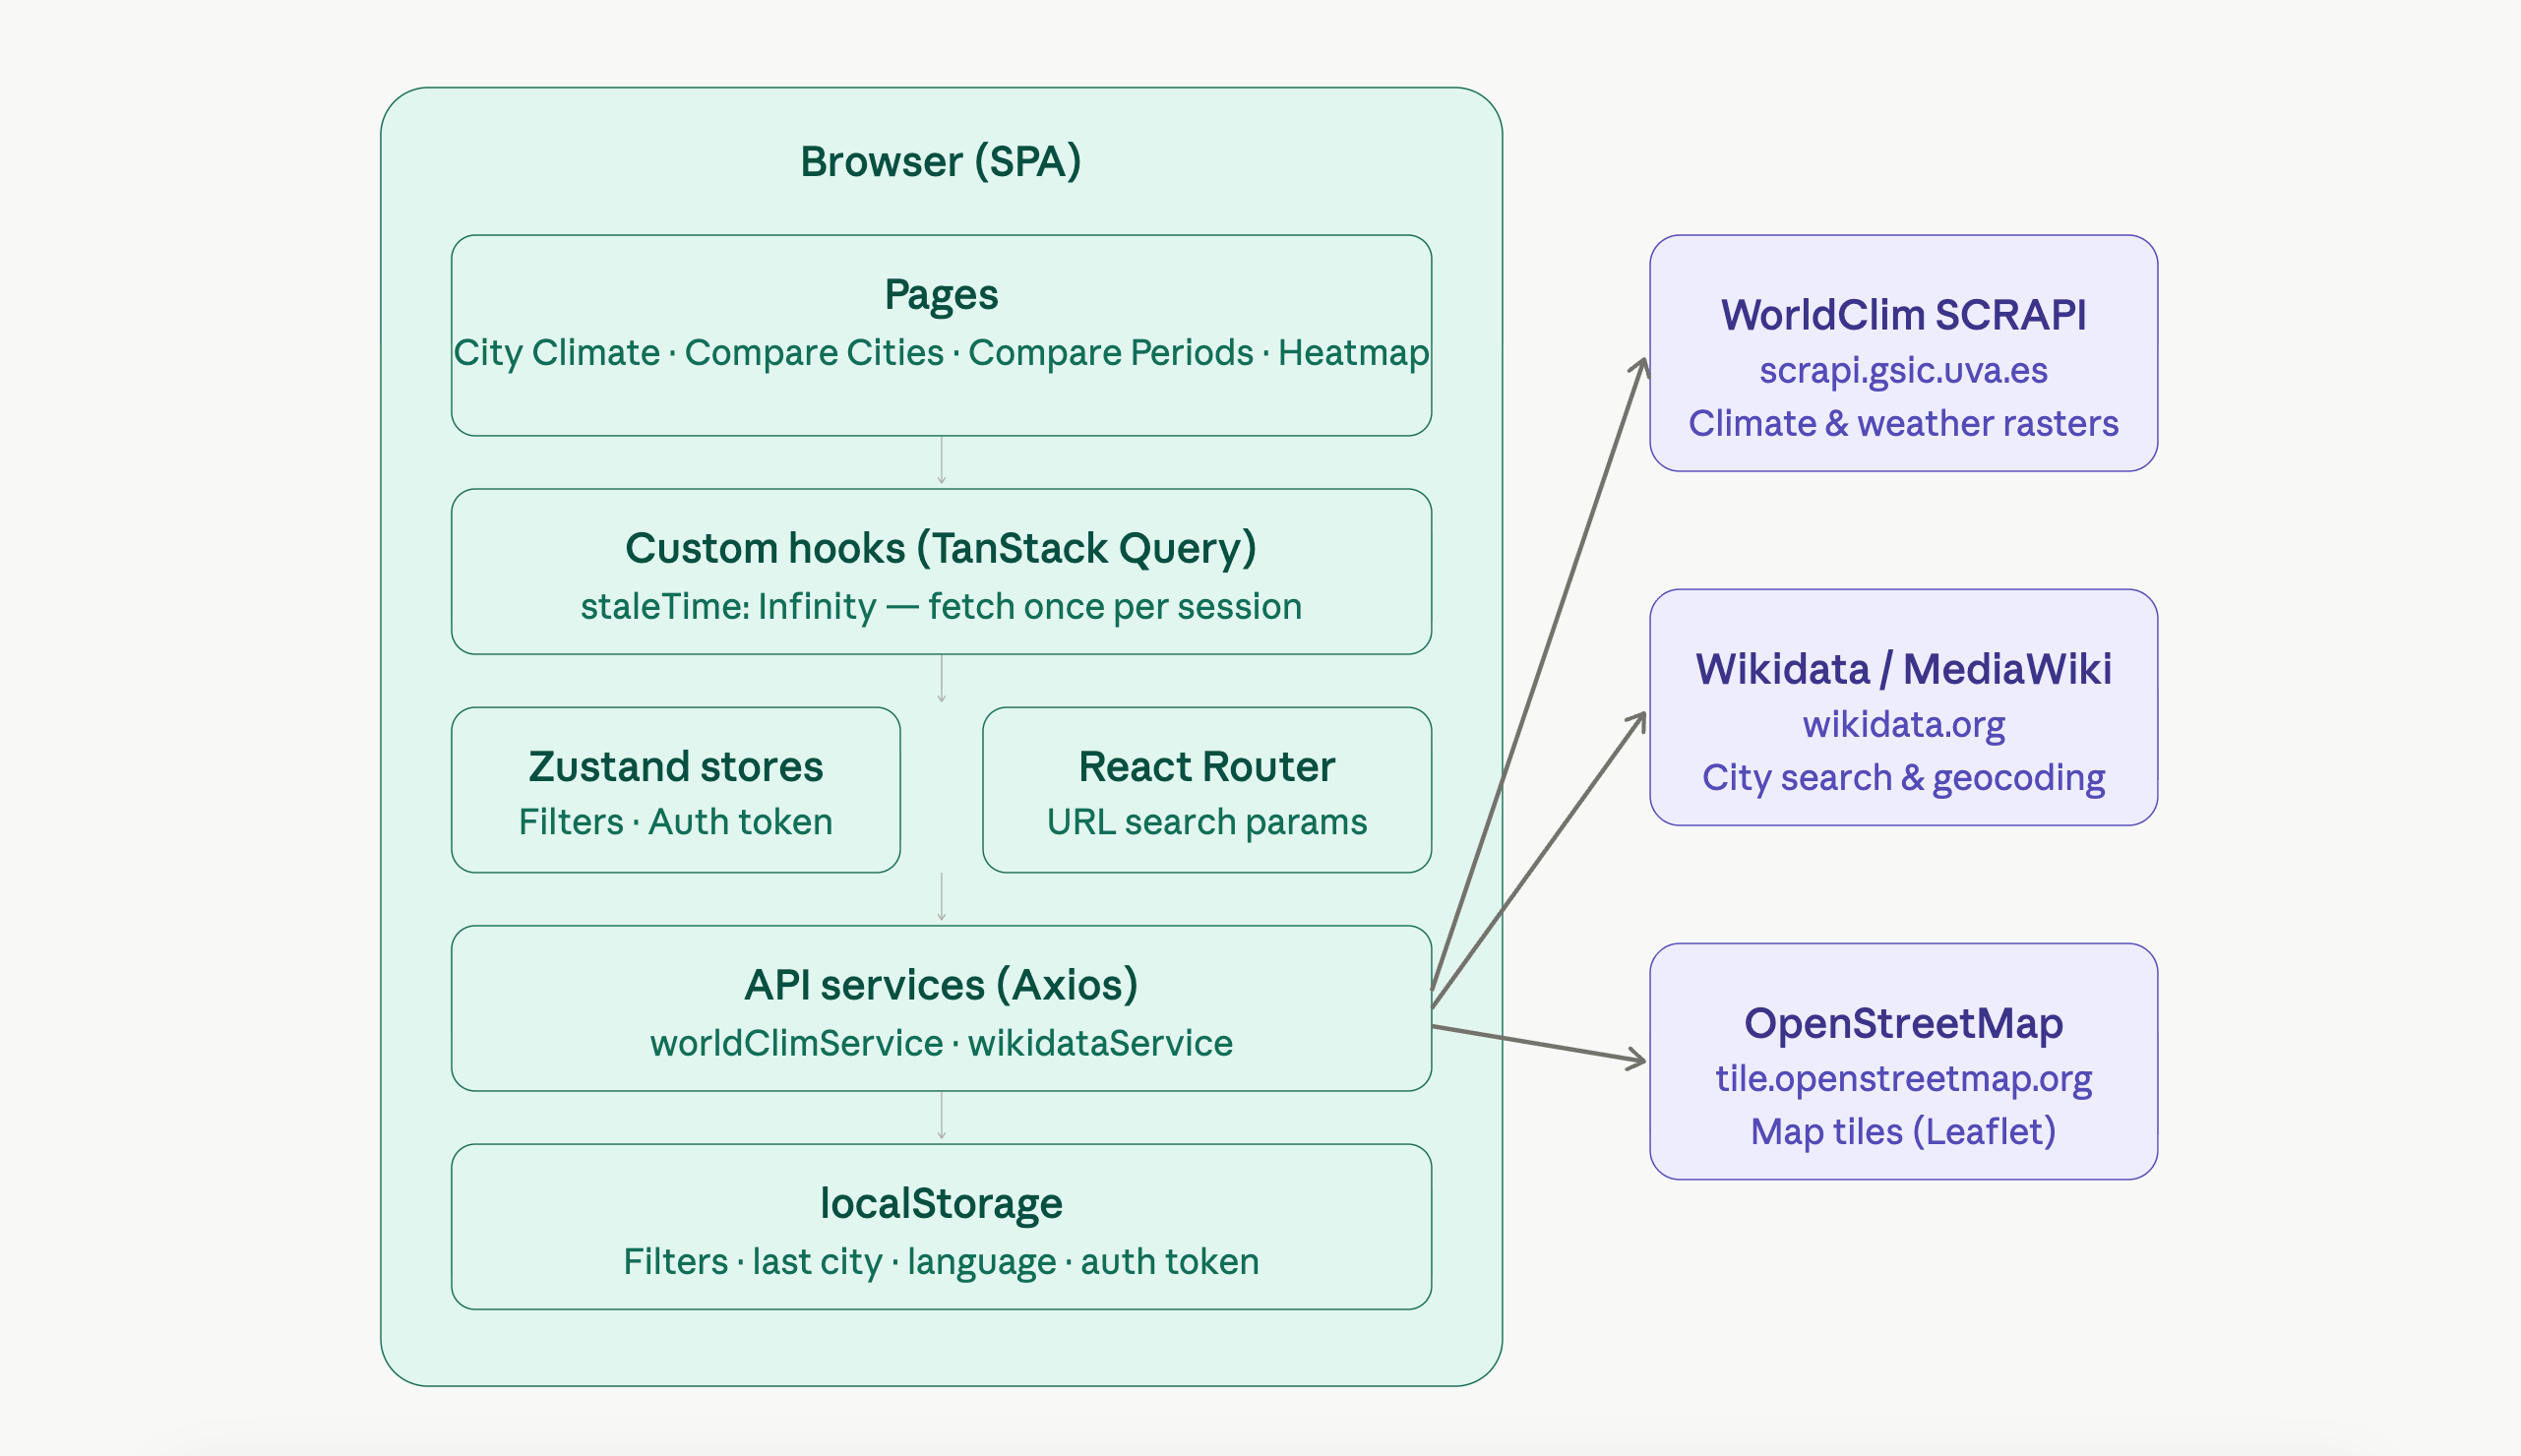
\includegraphics[width=\textwidth]{Images/climatica-architecture-v1.png}
  \caption{Original React SPA architecture (v1). All API calls originate in
    the browser. The WorldClim Bearer token is exposed as a client-side
    environment variable. City search is handled by the Wikidata pipeline.}
  \label{fig:arch_v1}
\end{figure}

The limitations described in Section~\ref{APP_ARCH_EVOLUTION} motivated a
redesign that introduced a server-side component, effectively superseding the
original client-side-only objective. The current architecture prioritises secure
API key handling, controllable city search ranking, and server-side caching over
the simplicity of a purely static deployment. Figure~\ref{fig:arch_v2} shows
the resulting Next.js full-stack architecture.

\begin{figure}[t]
  \centering
  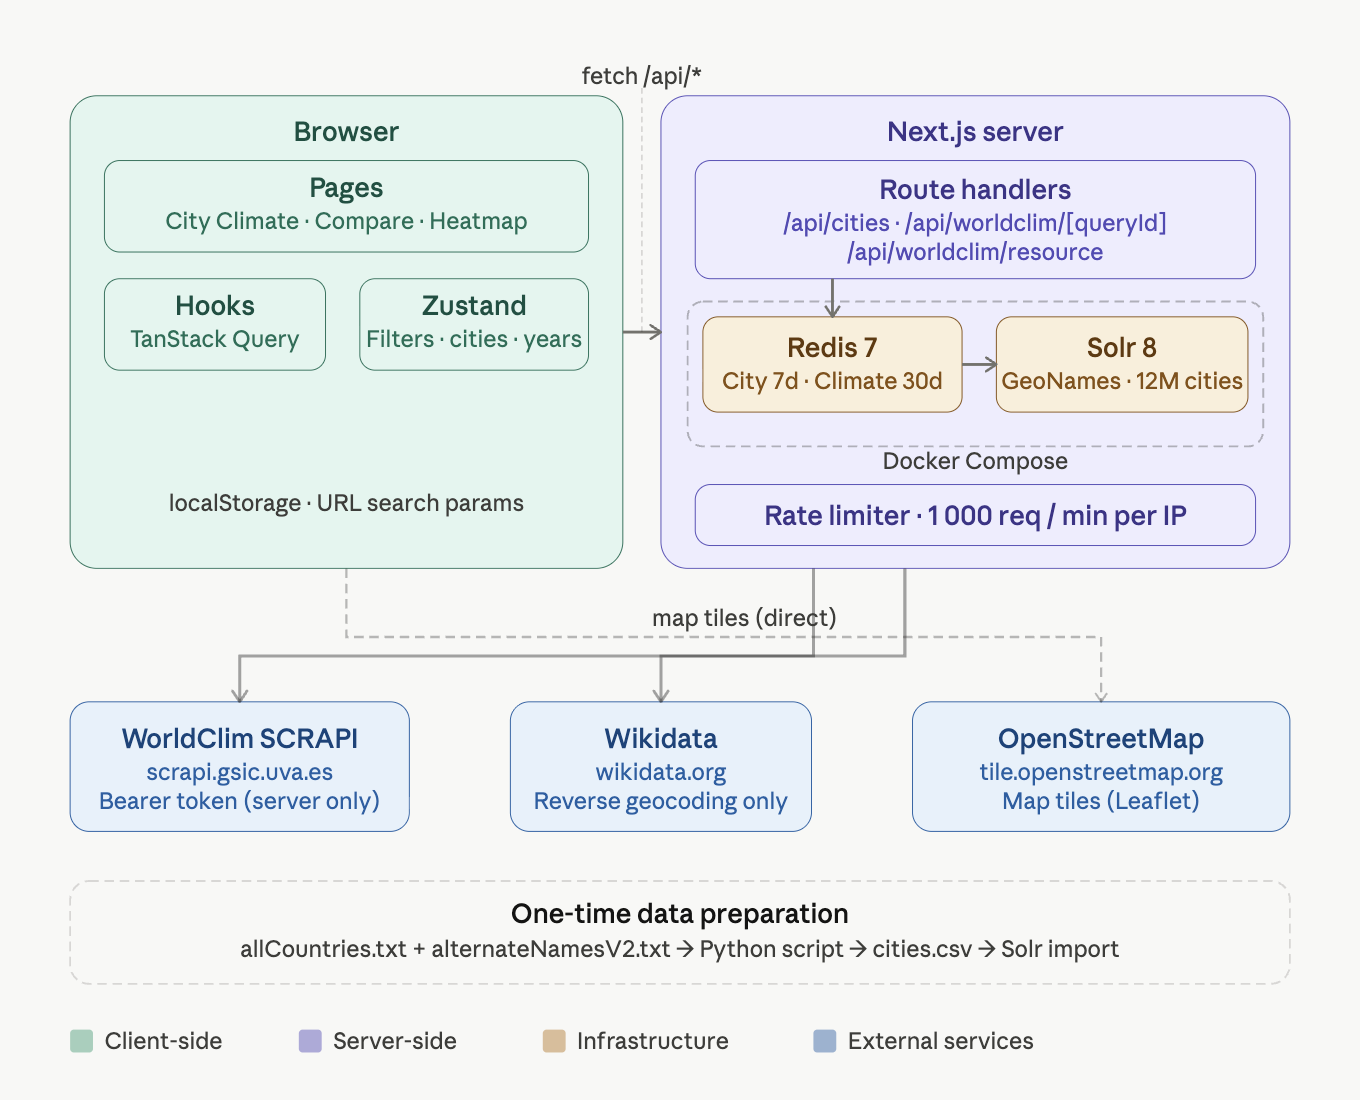
\includegraphics[width=\textwidth]{Images/climatica-architecture-v2.png}
  \caption{Next.js full-stack architecture (v2). The browser communicates only
    with Next.js route handlers. Redis caches Solr and SCRAPI responses
    server-side. The WorldClim Bearer token never reaches the client. Wikidata
    is retained for reverse geocoding (coordinate input and map clicks).
    Map tiles are fetched directly from OpenStreetMap by Leaflet.}
  \label{fig:arch_v2}
\end{figure}

The key components shown in Figure~\ref{fig:arch_v2} are: \textbf{Hooks}
(custom React hooks that manage data fetching via TanStack Query and expose
cached results to components); \textbf{Zustand} (a lightweight global state
store that persists filter settings, selected cities, and user preferences
across page navigations); \textbf{Redis} (a server-side in-memory cache that
stores responses from Solr and SCRAPI, reducing latency for repeated queries);
and \textbf{Solr~8} (the Apache Solr search index that powers city search over
12~million GeoNames records).

\subsection{City Search: from Wikidata to Solr}\label{APP_ARCH_SOLR}

In the original architecture, city search was implemented as a two-step
Wikidata pipeline described in Section~\ref{APP_ARCH_EVOLUTION}: a
\texttt{wbsearchentities} call followed by a SPARQL filter query. While this
approach required no local infrastructure, it was subject to Wikidata's
soft-throttling policy and offered no way to tune ranking without modifying
the SPARQL query.

The replacement pipeline uses GeoNames~\cite{geonames} as the data source.
GeoNames distributes two datasets: \texttt{allCountries.txt} (approximately
400\,MB, containing over 12~million place records with coordinates, feature
codes, and population figures) and \texttt{alternateNamesV2.txt} (approximately
200\,MB, containing localised place names in hundreds of languages).

A Python preprocessing script merges the two source files, filters records to
populated places only (GeoNames feature class \texttt{P}, covering the codes
\texttt{PPL}, \texttt{PPLA}, \texttt{PPLA2}--\texttt{PPLA5}, and \texttt{PPLC}),
and produces a single \texttt{cities.csv} file with one record per place
containing the GeoNames identifier, English, Ukrainian, and Spanish names,
coordinates, feature code, country code, and population. For the name fields,
the script applies a priority rule: the preferred alternate name for a given
language is taken first; if none exists, the ASCII name is used as fallback.

The resulting CSV is imported into an Apache Solr~8 core named
\texttt{cities}. The Solr schema defines three text fields for multilingual
name matching (\texttt{label\_en}, \texttt{label\_uk}, \texttt{label\_es})
and enables trigram-based sub-word indexing via a custom
\texttt{solrconfig.xml}. Trigrams allow partial-word matches: the query
\texttt{``val''} returns \texttt{Valladolid} without requiring a dedicated
prefix index or a minimum query length constraint.

For example, a query of \texttt{``mad''} matches \texttt{Madrid},
\texttt{Madeira}, and \texttt{Amadeus} --- the results are then ranked by
population so that the Spanish capital appears first. Exact prefix matches
receive a higher boost than trigram matches, ensuring that typing
\texttt{``Paris''} returns the French capital before smaller cities sharing
the same name.

At query time, the \texttt{SolrService} selects the label field that
corresponds to the active locale (\texttt{getLabelField}), constructs a
parameterised Solr query, and maps each document to a \texttt{TWikidataCity}
object that is compatible with the existing client-side data shapes. The query
is routed through the \texttt{/api/cities} Next.js route handler, which
consults Redis before forwarding to Solr.

Wikidata is still used for two closely related tasks: reverse geocoding when
the user clicks the map, and coordinate lookup when the user types a
latitude/longitude pair directly. Both cases call
\texttt{WikidataService.findNearestCityByCoordinates}, which issues a
GeoSearch request with a 10\,km radius. Because these operations are
low-frequency and point-in-time, the soft-throttling constraint that affects
interactive text search does not apply.

\subsection{Caching Strategy with Redis}\label{APP_ARCH_REDIS}

A Redis~7 instance provides server-side caching for all upstream requests.
The caching layer is implemented as a typed \texttt{RedisClient} singleton 
(using \texttt{ioredis}) with three distinct strategies defined in 
\texttt{REDIS\_STRATEGIES}:

\begin{itemize}
  \item \textbf{City search.} Results are cached by query string and language.
    Short queries (fewer than four characters) use a reduced Time-To-Live (TTL)
    because they produce broad result sets that become stale faster as the user
    continues typing. For longer queries, a per-key hit counter is incremented
    on every cache miss via a Redis \texttt{INCR} command; once a query crosses
    the \texttt{popularThreshold}, it is promoted to a longer TTL to retain
    frequently requested results in memory.

  \item \textbf{Climate data.} SCRAPI responses are cached by the full
    request URL. The same popularity-based TTL promotion applies: the first
    requests for a given location--period--variable combination use a standard
    30-day TTL; repeated requests extend the TTL automatically.

  \item \textbf{Nearest city (reverse geocoding).} Results are cached by
    rounded coordinate pair with a fixed TTL, since the nearest city to a
    given point does not change.
\end{itemize}

The \texttt{RedisClient} uses lazy connection, offline queuing, and
exponential-backoff retry (up to three attempts, at 100\,ms, 200\,ms, and
400\,ms) so that a Redis restart does not crash the application --- uncached
requests are simply served directly from Solr or SCRAPI until the connection
is restored.

Client-side, TanStack Query continues to operate with
\texttt{staleTime:~Infinity} for all WorldClim data, providing a second
caching layer within the browser session and preventing redundant calls to
the \texttt{/api/worldclim} route handlers.

\subsection{Infrastructure and Deployment}\label{APP_ARCH_INFRA}

Both Solr and Redis are managed through a single Docker Compose file at
\texttt{docker/docker-compose.yml}. The file defines two services:

\begin{itemize}
  \item \textbf{climatica-solr} --- Apache Solr~8 with a custom
    \texttt{solrconfig.xml} mounted from the repository. The container
    auto-creates the \texttt{cities} core on first start via the
    \texttt{solr-precreate} command entry point. A health check polls
    \texttt{/solr/cities/admin/ping} every 30 seconds with up to five
    retries.
  \item \textbf{climatica-redis} --- Redis~7 Alpine with append-only
    persistence (\texttt{redis-server --appendonly yes}) so that the
    cache survives container restarts. A health check runs
    \texttt{redis-cli ping} every 10 seconds.
\end{itemize}

Named volumes (\texttt{solr\_data}, \texttt{redis\_data}) persist index and
cache data across container lifecycles. The full developer workflow is
encapsulated in four \texttt{npm} scripts: \texttt{docker:up},
\texttt{docker:down}, \texttt{docker:reboot}, and \texttt{docker:logs}.
City data is imported into Solr via a two-step \texttt{npm run solr:reindex}
command that first POSTs the schema definition and then copies and imports the
\texttt{cities.csv} file into the running container. Indexing approximately
12~million records takes around three minutes on first run.

The application is deployed on a virtual server hosted at the Universidad de
Valladolid. The Next.js production server runs behind an Nginx reverse proxy
that handles SSL termination and forwards requests to the application process.
Climatica is publicly accessible at \url{https://climatica.gsic.uva.es/}.

\subsection{Folder Structure}\label{APP_ARCH_FOLDERS}

The Next.js source tree follows the App Router convention. The top-level
directories under \texttt{src/} are:

\begin{itemize}
  \item \texttt{app/} --- file-system routes. Each page directory contains
    a server component entry point and a client component view. The
    \texttt{app/api/} subdirectory contains the three route handlers:
    \texttt{cities/route.ts} (city search via Redis\,$\to$\,Solr),
    \texttt{worldclim/[queryId]/route.ts} (SCRAPI query proxy with rate
    limiting), and \texttt{worldclim/resource/route.ts} (SCRAPI resource
    proxy with Redis caching).

  \item \texttt{components/} --- shared UI components reused across pages,
    including the sidebar filter panel, chart components, skeleton loading
    placeholders, and the Leaflet map container (dynamically imported with
    \texttt{ssr:~false} to avoid the server-side rendering incompatibility
    of the Leaflet library).

  \item \texttt{hooks/} --- custom React hooks: \texttt{data/} for TanStack
    Query data-fetching hooks, \texttt{persisted/} for Zustand-backed
    state, and \texttt{ui/} for theme, geolocation, and drawing mode state.

  \item \texttt{libs/} --- server-only modules annotated with
    \texttt{import "server-only"}: \texttt{redis/} (client singleton and
    caching strategies), \texttt{api/} (Axios instance), and
    \texttt{services/} (\texttt{SolrService}, \texttt{WikidataService},
    \texttt{WorldClimService}).

  \item \texttt{types/}, \texttt{constants/}, \texttt{utils/} --- pure
    TypeScript with no framework imports. All magic values are declared as
    named constants; naming follows a strict convention: \texttt{T} prefix
    for types, \texttt{E} prefix for enums, \texttt{*.constant.ts} for
    constants.
\end{itemize}

\subsection{Data Flow}\label{APP_ARCH_FLOW}

The data flow follows a strict unidirectional pattern:

\begin{center}
\texttt{Component \textrightarrow\ Hook \textrightarrow\ fetch /api/* \textrightarrow\
Route Handler \textrightarrow\ Redis \textrightarrow\ Solr / SCRAPI}
\end{center}

Client components never call external services directly --- all requests go
through \texttt{/api/} route handlers. This boundary ensures that
authentication credentials remain server-side and that the Redis cache is
always consulted before any upstream request is made.

\subsection{State Management}\label{APP_ARCH_STATE}

State is stratified by lifetime and sharing scope, as shown in
Table~\ref{tab:state}. This stratification avoids the common anti-pattern of
storing everything in a single global store, which makes it difficult to reason
about what triggers re-renders and why.

\begin{table}[H]
  \centering
  \caption{State management strategy in Climatica.}
  \label{tab:state}
  \begin{adjustbox}{width=1.2\textwidth,center}
    \small
    \begin{tabular}{p{4cm}p{3.5cm}p{7cm}}
      \toprule
      \textbf{State type} & \textbf{Location} & \textbf{Rationale} \\
      \midrule
      Server data (WorldClim, Solr) & TanStack Query &
        Automatic deduplication; \texttt{staleTime: Infinity} since climate
        data never changes \\
      Global filter settings & Zustand + \texttt{persist} &
        Survives page navigation; persisted to \texttt{localStorage} \\
      Selected weather years & Zustand + \texttt{persist} &
        Up to five years retained across sessions \\
      City sync setting & Zustand + \texttt{persist} &
        Opt-out toggle; default on \\
      Shareable UI state & URL search params &
        Allows bookmarking and sharing specific views \\
      Last selected city & \texttt{usePersistedCity} hook &
        Survives hard reload without polluting URL \\
      Comparison cities & \texttt{usePersistedComparisonCities} hook &
        Separate store for City~A / City~B \\
      UI-only state & Local \texttt{useState} &
        Scoped to component; no need to share \\
      Derived data & Computed at render time &
        Never stored; computed from props or query results \\
      \bottomrule
    \end{tabular}
  \end{adjustbox}
\end{table}

\textbf{Cross-page city synchronisation.} A configurable sync feature
propagates the selected city across pages when enabled. The setting is stored
in the Zustand \texttt{filtersStore} under the key \texttt{syncCity}
(default: on) and is toggled via a \texttt{ToggleSwitch} in a collapsible
Settings section of the sidebar. When the user selects a city on any page,
the sync logic updates both \texttt{usePersistedCity} (used by City Climate
and Compare Periods) and \texttt{usePersistedComparisonCities.cityA} (used
by Compare Cities), so that the selected city immediately appears as the
primary city on all other pages. City~B on Compare Cities is never synced ---
only City~A participates in the cross-page propagation. The sync is guarded
by a \texttt{hasHydrated} flag that prevents race conditions during the
initial Zustand store rehydration from \texttt{localStorage}.

\subsection{Draft Filter Pattern}\label{APP_ARCH_DRAFT}

The global sidebar maintains a \emph{draft} copy of the filter state separate
from the committed Zustand store. Users adjust chips and dropdowns freely; the
draft is validated with Zod and committed to the store only when the user clicks
``Apply filters''. This prevents partial or invalid filter states from triggering
expensive API calls mid-edit.

The draft also enforces domain constraints eagerly: switching the dataset to
\emph{Weather} automatically strips the three variables unavailable in that
dataset (\texttt{srad}, \texttt{wind}, \texttt{vapr}) and downgrades the
30-second grid to 2.5-minute resolution, because weather rasters are not
available at 30-second resolution.

\subsection{Skeleton Loading States}\label{APP_ARCH_SKELETONS}

Every section of the interface that depends on asynchronous data has a
dedicated skeleton loading placeholder. Five skeleton components --- all
using Tailwind CSS~\cite{tailwindcss} \texttt{animate-pulse}
class --- cover the main content areas:
\texttt{ChartSkeleton} (a twelve-bar animated placeholder that matches the
approximate shape of a real climate chart), \texttt{MapSkeleton} (a tile-grid
layout with a centre pin indicator, available in \texttt{full} and
\texttt{mini} variants), \texttt{StatCardsSkeleton} (a responsive grid of
blank stat cards), \texttt{TableSkeleton} (a configurable table with a header
row and body rows), and \texttt{ComparisonTableSkeleton} (a fixed five-row
variant for the comparison stats grid).

Figure~\ref{fig:skeleton_loading} shows the Compare Cities page in its loading
state, where the minimap, statistics table, and chart are all replaced with
animated placeholders until data arrives from the route handlers.

\begin{figure}[t]
  \centering
  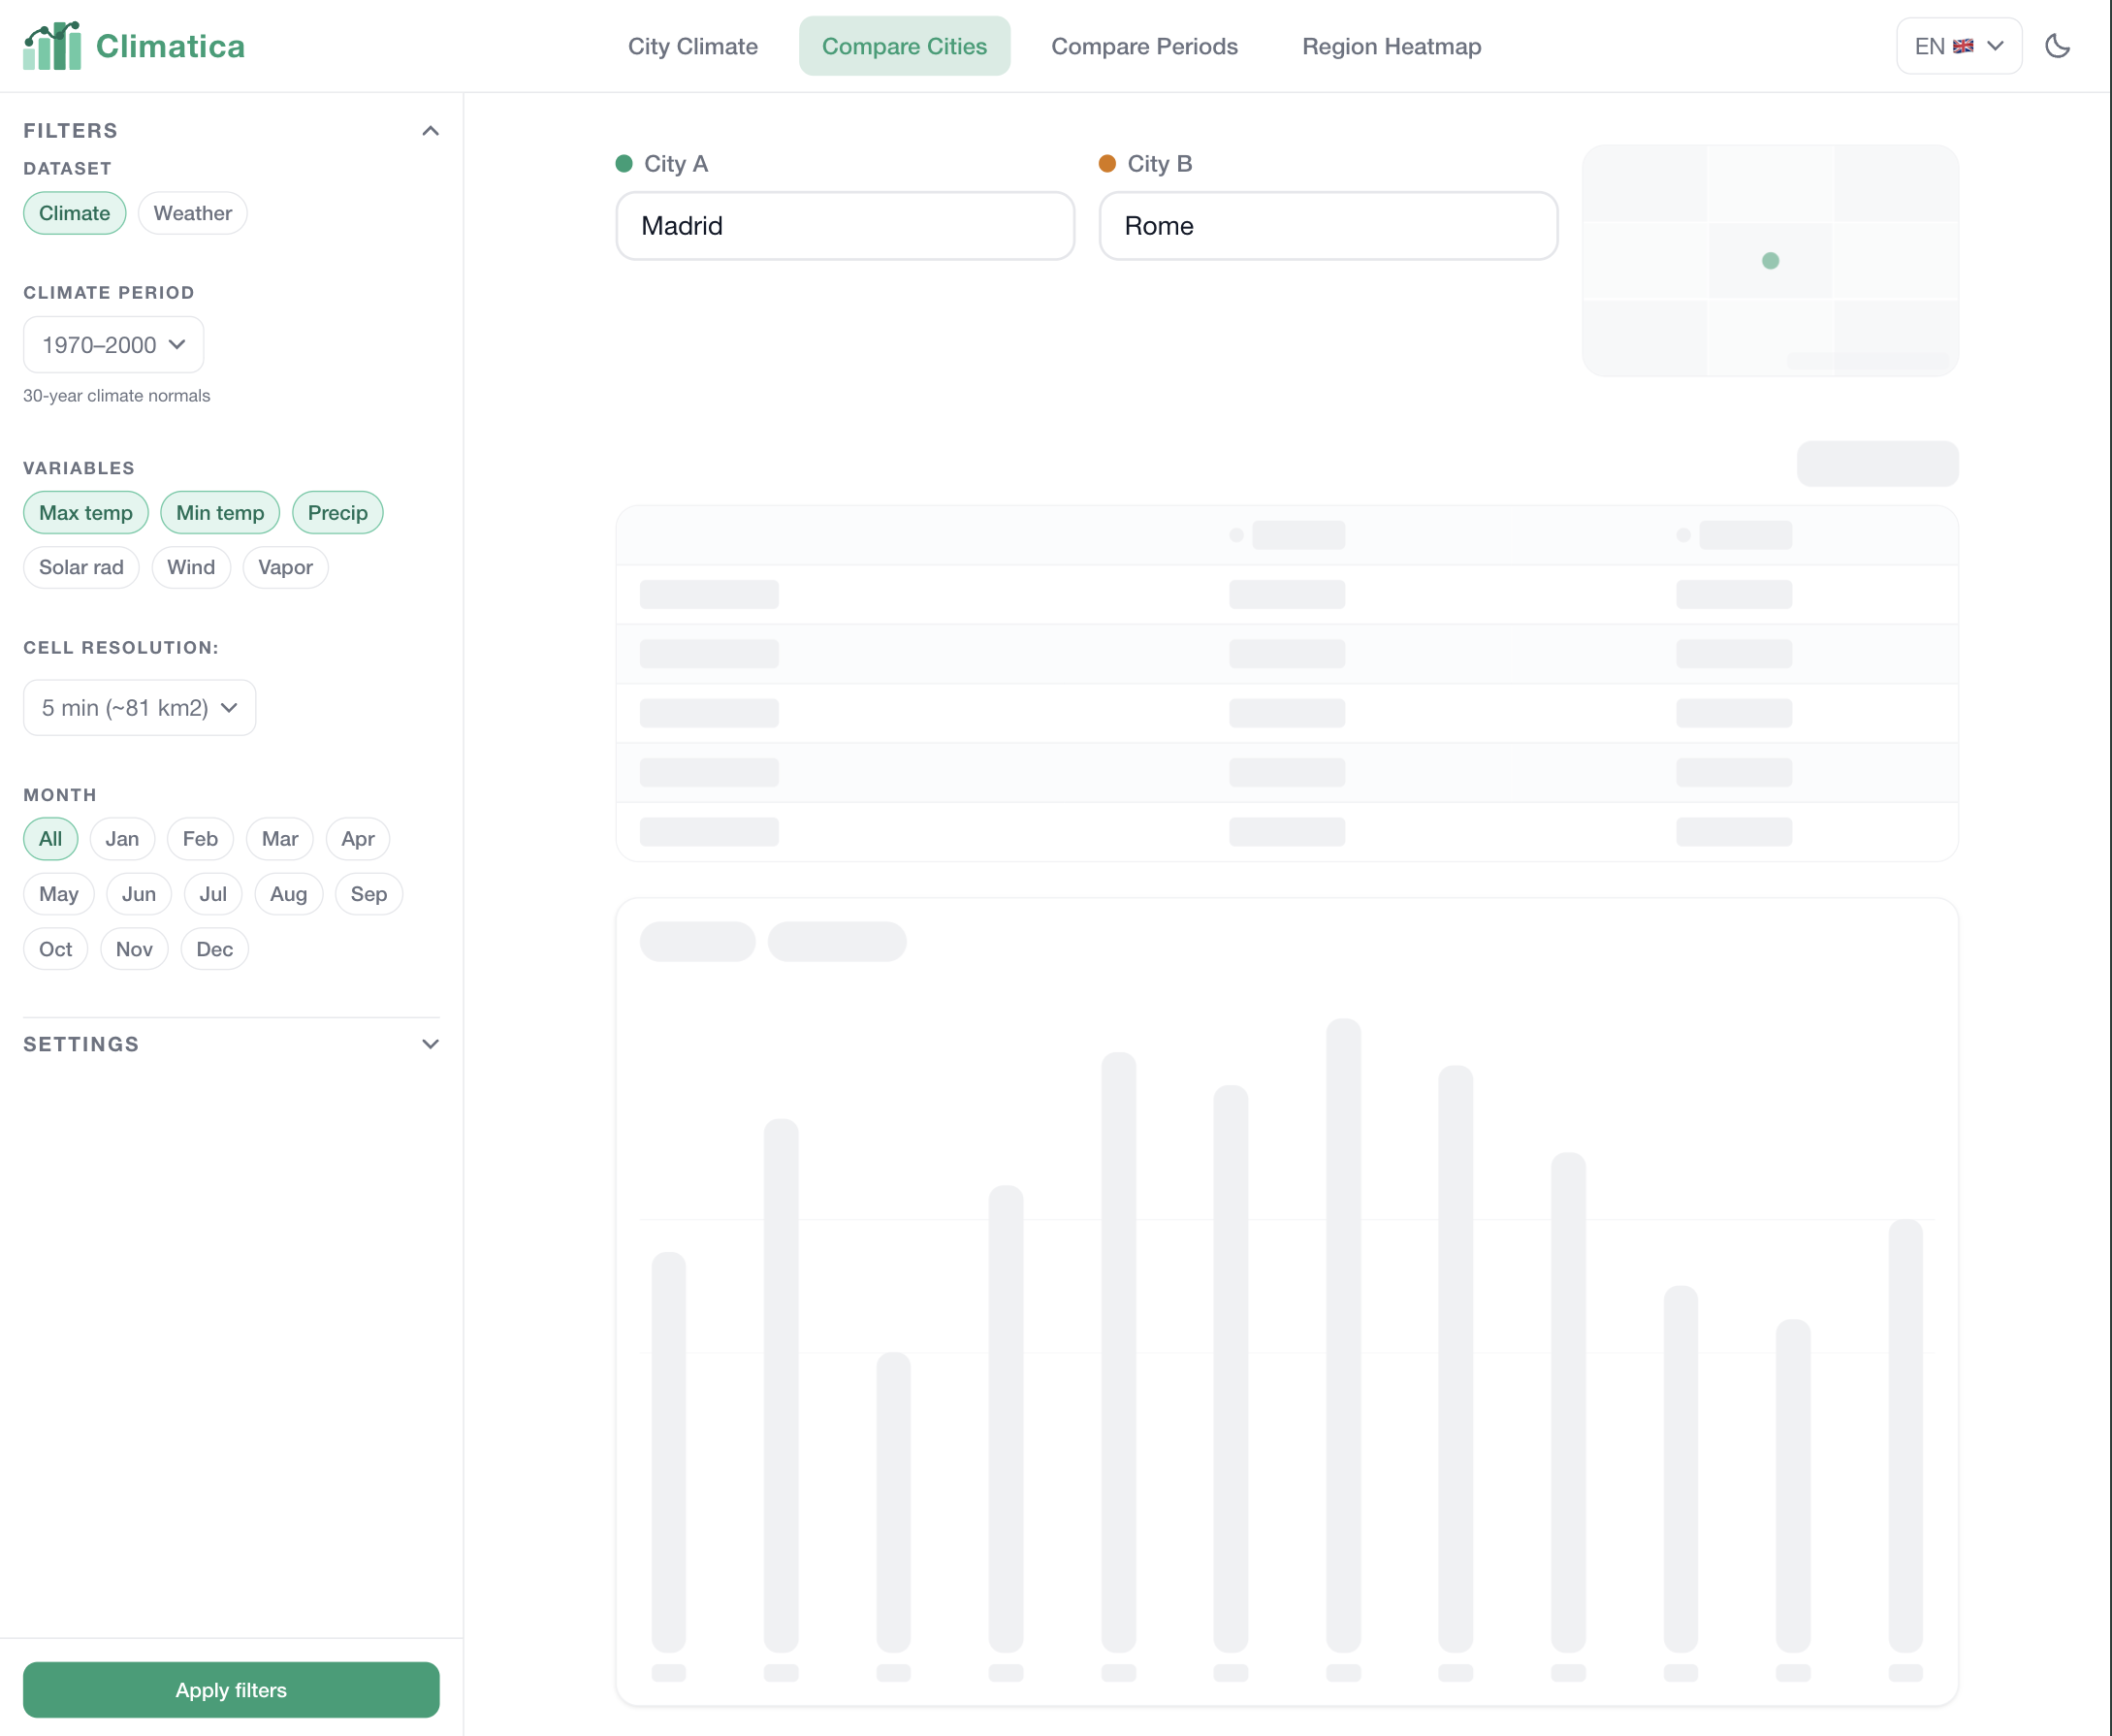
\includegraphics[width=0.9\textwidth]{Images/climatica-skeleton-loading-state.png}
  \caption{Compare Cities page in its loading state. The minimap, statistics
    table, and chart are replaced with animated skeleton placeholders. The map
    skeleton uses a tile-grid pattern with a central pin to mimic the appearance
    of a Leaflet map.}
  \label{fig:skeleton_loading}
\end{figure}

Climatica uses Leaflet~\cite{leaflet} for all interactive map rendering.
Leaflet is a client-side JavaScript library that depends on the browser
\texttt{window} object and therefore cannot be server-side rendered. All
Leaflet map components (\texttt{LeafletMap}, \texttt{MapCanvas},
\texttt{MiniMap}) are dynamically imported with \texttt{ssr:~false} and use
\texttt{MapSkeleton} as their loading fallback, which prevents a server-side
rendering crash. In weather mode on the Compare Periods page, each year column
in the \texttt{MultiPeriodStatsTable} displays an individual skeleton
placeholder while its TanStack Query is still in-flight, so partial results
become visible progressively rather than blocking the entire table.

\subsection{Data Transformation and Domain Logic}\label{APP_ARCH_LOGIC}

A critical aspect of Climatica is the transformation of raw SCRAPI results into
meteorologically sound data structures. Unlike typical CRUD applications,
Climatica performs significant client-side computation to ensure scientific
accuracy.

\textbf{Aridity Calculation.} Following the Gaussen-Walter-Lieth climate
classification, a month is defined as arid when $P < 2T$, where $P$ is
precipitation in mm and $T$ is average temperature in $^\circ$C. This condition
is evaluated per month in \texttt{computeAridityPeriods} and is used both to
colour the bars in the standard climograph and to drive the filled areas in the
Walter-Lieth diagram.

\textbf{Dynamic Axis Scaling.} To maintain the $1{:}2$ ratio visually, the
application implements a custom scaling engine in \texttt{getWalterLiethScales}
(Listing~\ref{lst:scaling}). The algorithm ensures that both axes share the
same zero-baseline, that the precipitation maximum is exactly twice the
temperature maximum, and that tick values are rounded to the nearest multiple
of 5 for readability.

\begin{lstlisting}[language=TypeScript,
  caption={Walter-Lieth axis synchronisation.},
  label={lst:scaling}]
export function getWalterLiethScales(
  data: TMonthlyTemperature[]
): TWalterLiethScales {
  const tMax = Math.max(...data.map(d => (d.tmin + d.tmax) / 2));
  const tempMax = Math.ceil(tMax / 5) * 5;
  return {
    tempMin: 0, tempMax,
    precMin: 0, precMax: tempMax * 2,
  };
}
\end{lstlisting}

\subsection{Advanced SVG Visualisation}\label{APP_ARCH_SVG}

Implementing the Walter-Lieth climatogram in a browser-based application
presented several non-trivial engineering challenges, because standard charting
libraries such as Recharts are designed for non-overlapping datasets and do not
natively support the intersection-fill pattern required by the Walter-Lieth
convention.

The core difficulty is that the arid and humid fills are not simply the area
under each curve: they are the regions where one curve is \emph{above} the
other, which means the fill boundaries change at every crossing point of the
two curves. A naïve approach --- drawing a blue rectangle wherever precipitation
exceeds temperature and an orange one wherever temperature exceeds precipitation
--- fails because the two filled regions overlap at the crossing points,
producing visible artefacts.

The solution uses SVG \texttt{clipPath} with the \textbf{even-odd winding rule}.
Two closed SVG paths are constructed --- $\mathit{Area}_T$ (the region from the
temperature curve down to the baseline) and $\mathit{Area}_P$ (the corresponding
precipitation region). A composite \texttt{clipPath} is built by concatenating
both paths. Because the even-odd rule fills a point only if it is enclosed by an
\emph{odd} number of component paths, the intersection region (where both curves
overlap) is automatically excluded from each fill. The result is pixel-perfect
arid and humid shading with no artefacts and no need to compute spline
intersection points explicitly.

The temperature and precipitation curves are rendered using Catmull-Rom spline
interpolation rather than straight line segments, which produces the smooth,
organic appearance characteristic of traditional Walter-Lieth diagrams.

Coordinate projection relies on Recharts~v3 internal hooks
(\texttt{useXAxisScale}, \texttt{useYAxisScale}), which expose the D3 scale
functions used internally by the chart. The custom \texttt{WLCustomized}
component uses these scales to convert data-space values into SVG pixel
coordinates, making the overlay fully responsive to window resizing.


% ─── 3.3 Justification of Technology Choices ───────────────────────────────────────────────────
\section{Justification of Technology Choices}\label{APP_TECH}

The architecture described in Section~\ref{APP_ARCH} relies on a number of
specific technologies. This section summarises the rationale for the most
significant choices, comparing each selected technology to the alternatives
that were considered and explaining why it was preferred.

Table~\ref{tab:tech} lists the full technology stack with versions and roles.

\begin{table}[H]
  \centering
  \caption{Technology stack of Climatica (v2).}
  \label{tab:tech}
  \small
  \begin{tabular}{llp{6.5cm}}
    \toprule
    \textbf{Technology} & \textbf{Version} & \textbf{Role} \\
    \midrule
    Next.js        & 16.2  & Full-stack framework; App Router; server-side
                             route handlers \\
    React          & 19.2  & Component model and declarative UI \\
    TypeScript     & 5.x   & Static typing with strict mode \\
    Tailwind CSS   & 4.2   & Utility-first styling \\
    TanStack Query & 4.43  & Client-side server-state management and
                             deduplication \\
    Zustand        & 5.0   & Lightweight global client state with
                             \texttt{persist} middleware \\
    Zod            & 4.3   & Runtime validation of filter inputs \\
    next-intl      & 4.12  & Internationalisation across three locales \\
    Leaflet + react-leaflet & 1.9 / 5.0 & Interactive map rendering \\
    Recharts       & 3.8   & SVG chart rendering; coordinate hooks for
                             Walter-Lieth overlay \\
    Axios          & 1.13  & HTTP client for client-side API calls \\
    Apache Solr    & 8     & City search index with trigram tokenisation \\
    Redis          & 7     & Server-side response cache \\
    ioredis        & 5.10  & Type-safe Redis client with retry logic \\
    html2canvas    & 1.4   & DOM-to-canvas rasterisation for PNG export \\
    Vitest         & 4.x   & Unit test runner \\
    Playwright     & 1.60  & End-to-end browser testing \\
    Docker Compose & ---   & Local orchestration of Solr and Redis \\
    \bottomrule
  \end{tabular}
  \normalsize
\end{table}

\textbf{Next.js.} The migration from Vite to Next.js was motivated by two
architectural requirements that a static SPA cannot satisfy: server-side route
handlers (needed to keep the WorldClim Bearer token off the client and to
front-run requests with Redis) and a richer deployment target that runs on the
university server alongside Nginx. The App Router model maps naturally to the
four-page structure of Climatica, and the clear server/client component boundary
makes it explicit which code runs where.

\textbf{Apache Solr.} Solr was chosen over alternatives (PostgreSQL full-text
search, Elasticsearch, Meilisearch) because it is mature, has first-class
support for trigram tokenisation via \texttt{solrconfig.xml} customisation, and
runs comfortably within the memory budget of the university server. The trigram
analyser enables partial-word matching --- a user typing \texttt{``mad''} sees
\texttt{Madrid} immediately --- without requiring a dedicated prefix index.

\textbf{Redis.} Redis was preferred over in-process caches because it persists
across server restarts and is shared across all Next.js worker processes. The
popularity-based TTL promotion strategy, which extends cache lifetime for
frequently requested queries, relies on an \texttt{INCR} counter that would not
be possible with a process-local cache.

\textbf{next-intl.} The original i18next integration was replaced by next-intl,
which integrates natively with the Next.js App Router middleware layer. Language
detection and locale routing are handled at the edge, so the correct locale is
available server-side on every request without a client-side hydration step.

\textbf{Vitest and Playwright.} Vitest was chosen over Jest for unit tests
because it shares the same ESM configuration as the rest of the project,
eliminating the need for a separate Babel transform. Playwright was chosen for
E2E tests because it supports all major browsers from a single configuration,
runs headlessly in CI with minimal setup, and provides a visual trace viewer
(\texttt{test:e2e:ui}) that makes debugging failed tests significantly faster.


% ─── 3.4 Quality Assurance ────────────────────────────────────────────────────
\section{Quality Assurance}\label{APP_QA}

\subsection{Testing Strategy}\label{APP_QA_TESTS}

The test suite is divided into two layers with clearly separated
responsibilities.

\textbf{Unit tests} are written with Vitest and cover the server-side modules
that contain the most business-critical logic: the Redis client and all three
caching strategies, the \texttt{/api/cities} and \texttt{/api/worldclim} route
handlers, \texttt{SolrService}, \texttt{WorldClimService}, URL utility functions,
and the city description generator. These tests run against mocked dependencies
and do not require Docker to be running, which keeps the feedback cycle fast
during development. Running \texttt{npm run test:coverage} produces a V8
coverage report that makes untested code paths immediately visible.

\textbf{End-to-end tests} are written with Playwright and cover five
user-visible flows: city search and result selection, climate data loading and
chart rendering, language switching across the three supported locales,
cross-page navigation, and the 404 not-found page. E2E tests require both
Docker services to be running and the Next.js development server to be active.

\subsection{CI/CD Pipelines}\label{APP_QA_CICD}

Two GitHub Actions workflows run on every push and pull request to the main
branch.

The \textbf{validation and build} pipeline executes the quality gate in
sequence: TypeScript compilation (\texttt{tsc --noEmit}), ESLint, Prettier
format check, unit tests with coverage, and a production build
(\texttt{next build}). This pipeline must pass before any merge is permitted.

The \textbf{E2E tests} pipeline spins up the Docker Compose stack (Solr and
Redis), waits for both health checks to pass, starts the Next.js server, and
then runs the full Playwright suite. Running E2E tests in CI catches regressions
in the full request path --- including route handler logic, Redis cache
behaviour, and Solr query construction --- that unit tests cannot detect in
isolation.

Together the two pipelines provide the safety net required for confident,
incremental deployment to the Universidad de Valladolid server.


% ─── 3.5 Prototype Description ────────────────────────────────────────────────
\section{Prototype Description}\label{APP_PROTO}

Climatica is organised into four pages accessible from the top navigation bar.
All pages share a persistent left sidebar containing the global filter controls.
The application supports light and dark themes; all screenshots in this section
show the light theme.

\subsection{City Climate}\label{APP_PROTO_CITY}

The City Climate page (Figure~\ref{fig:page_city_map}) is the primary entry
point of the application. The user searches for a city by name (backed by the
Solr index), enters coordinates directly, clicks a point on the map, or uses
the browser geolocation button. Upon selection, the page displays an interactive
Leaflet map centred on the selected city, with a pin marking the exact location
and a dashed rectangle outlining the WorldClim raster cell being queried,
together with four summary stat cards (average maximum temperature, average
minimum temperature, total annual precipitation, and elevation). Below the map,
the user can switch between two chart modes:

\begin{itemize}
  \item \textbf{Standard climograph} (Figure~\ref{fig:page_city_std}) ---
    precipitation as vertical bars (blue for humid months, yellow for arid
    months) and temperature as smooth lines.
  \item \textbf{Walter-Lieth diagram} (Figure~\ref{fig:page_city_wl}) ---
    precipitation and temperature as two smooth curves with filled areas
    indicating arid (yellow) and humid (blue) periods.
\end{itemize}

\begin{figure}[t]
  \centering
  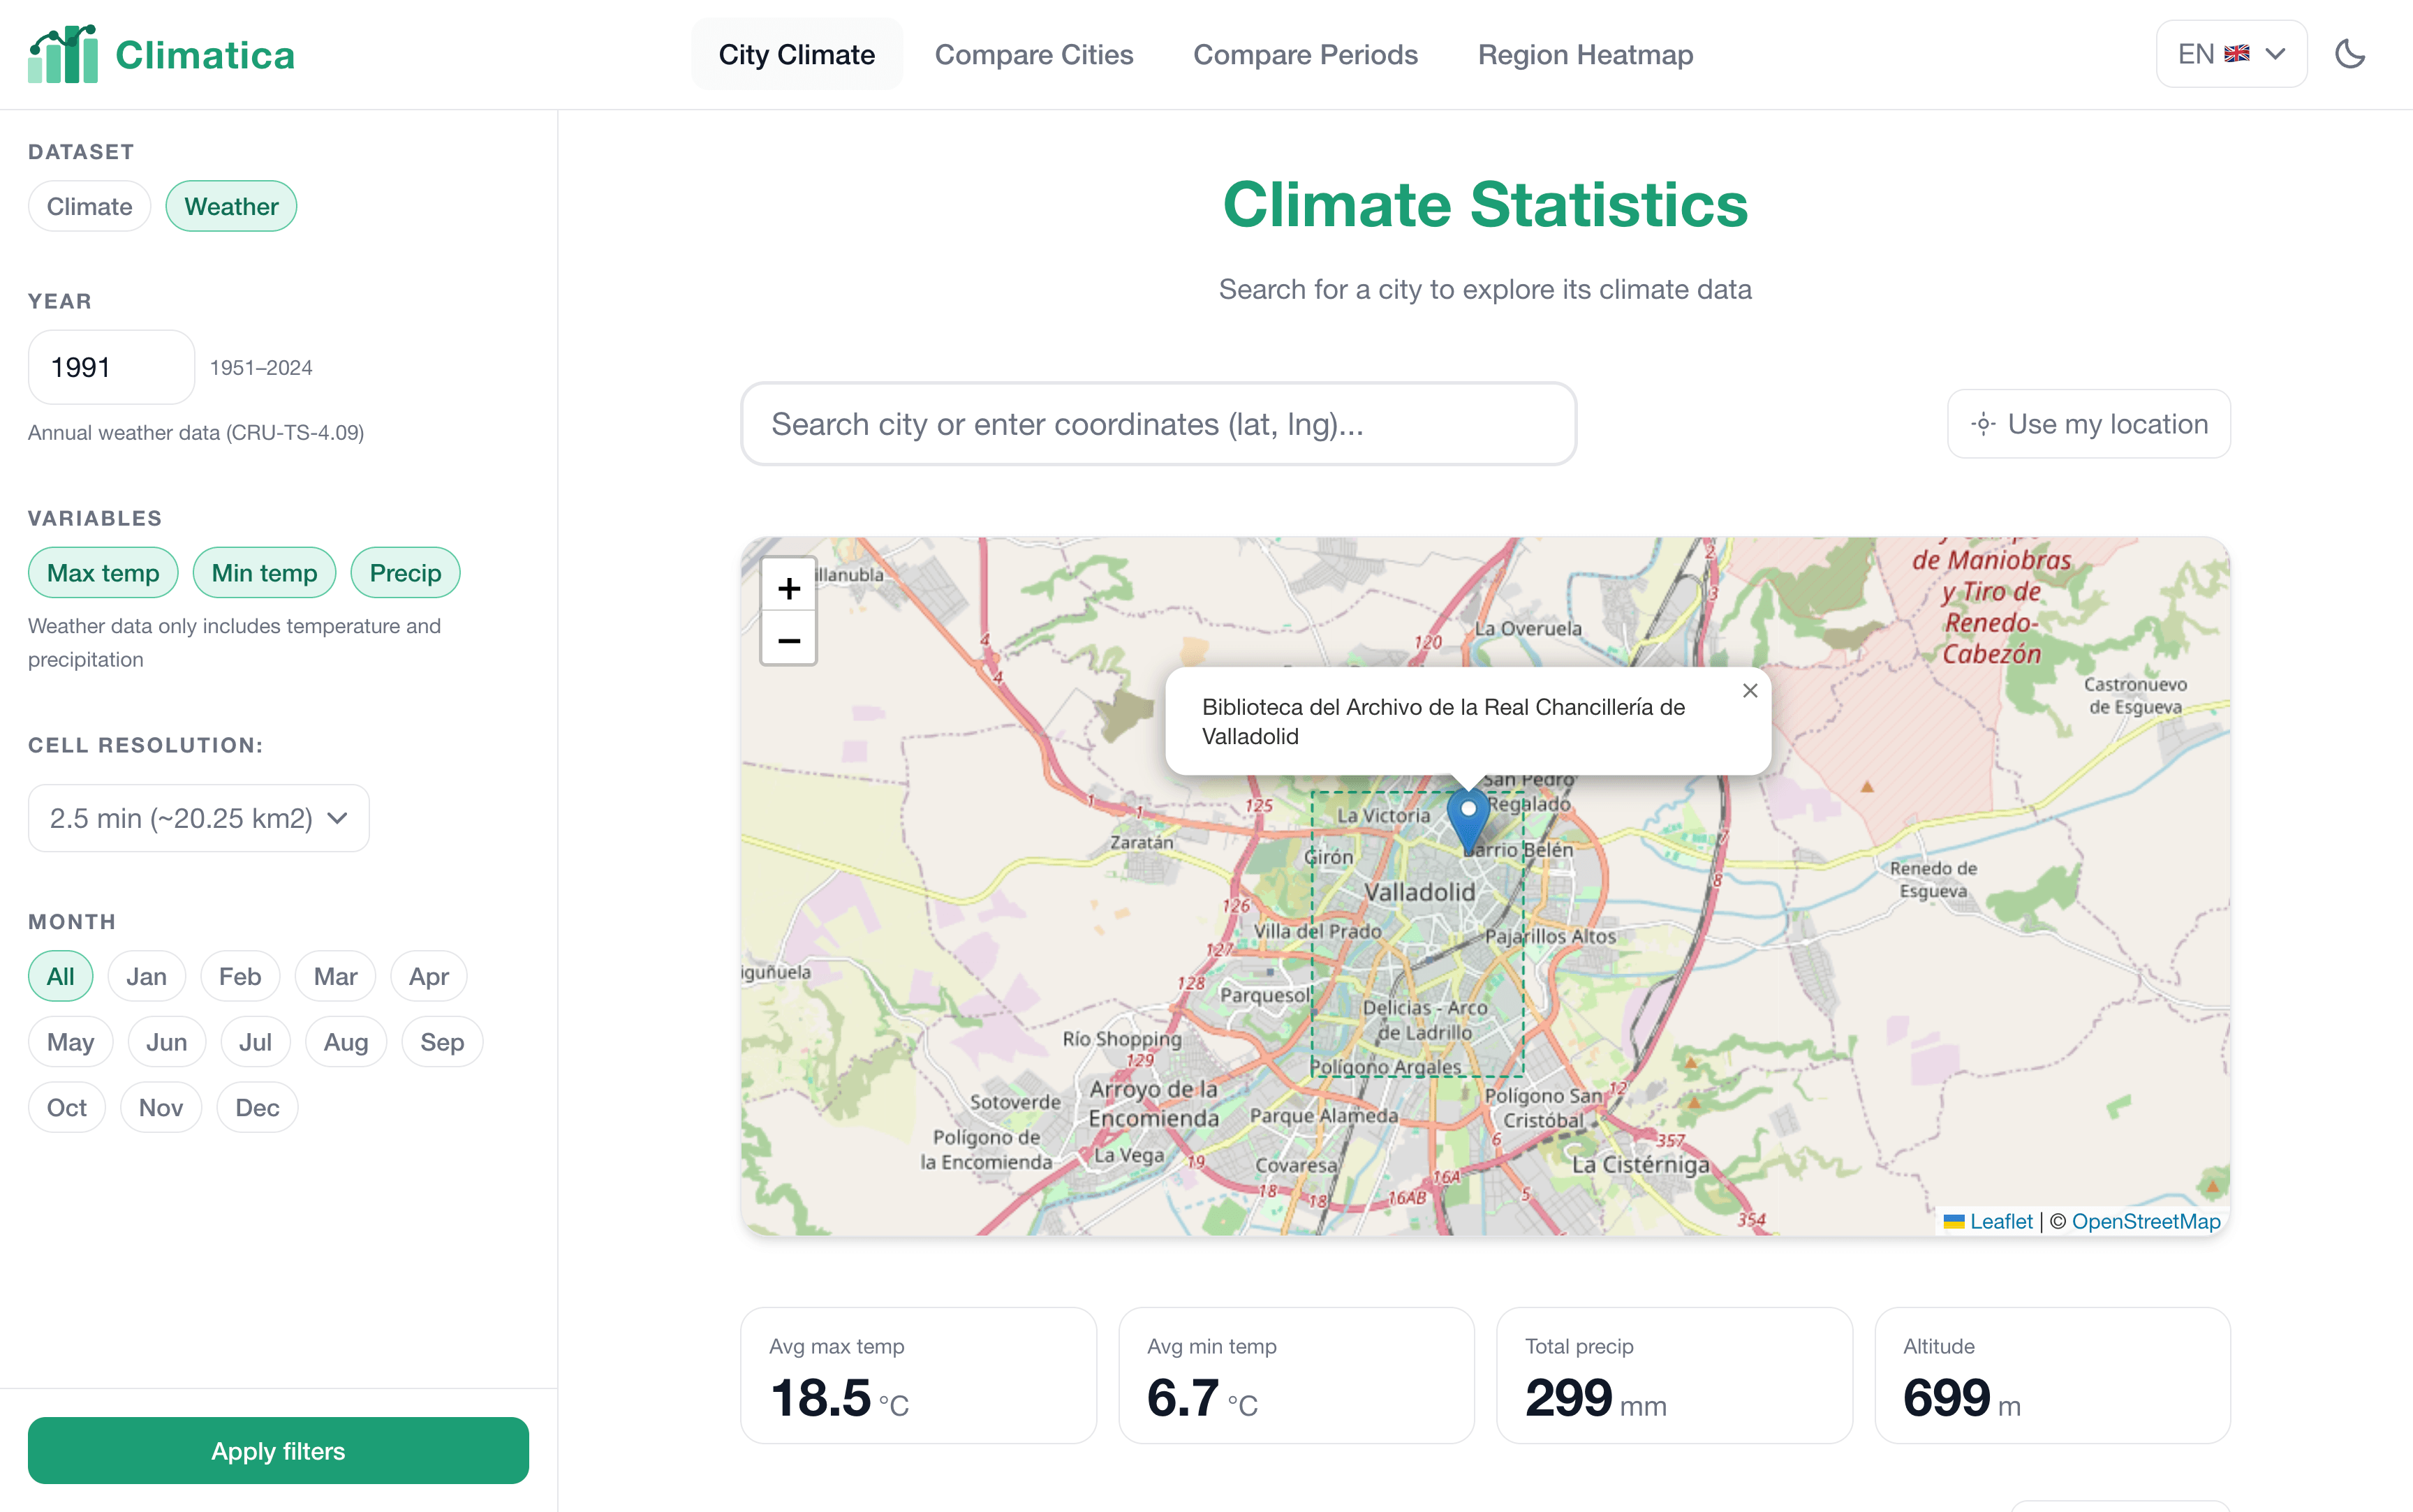
\includegraphics[width=0.9\textwidth]{Images/climatica-map.png}
  \caption{City Climate page --- map view with location pin, raster cell
    outline, and summary stat cards for Valladolid.}
  \label{fig:page_city_map}
\end{figure}

\begin{figure}[t]
  \centering
  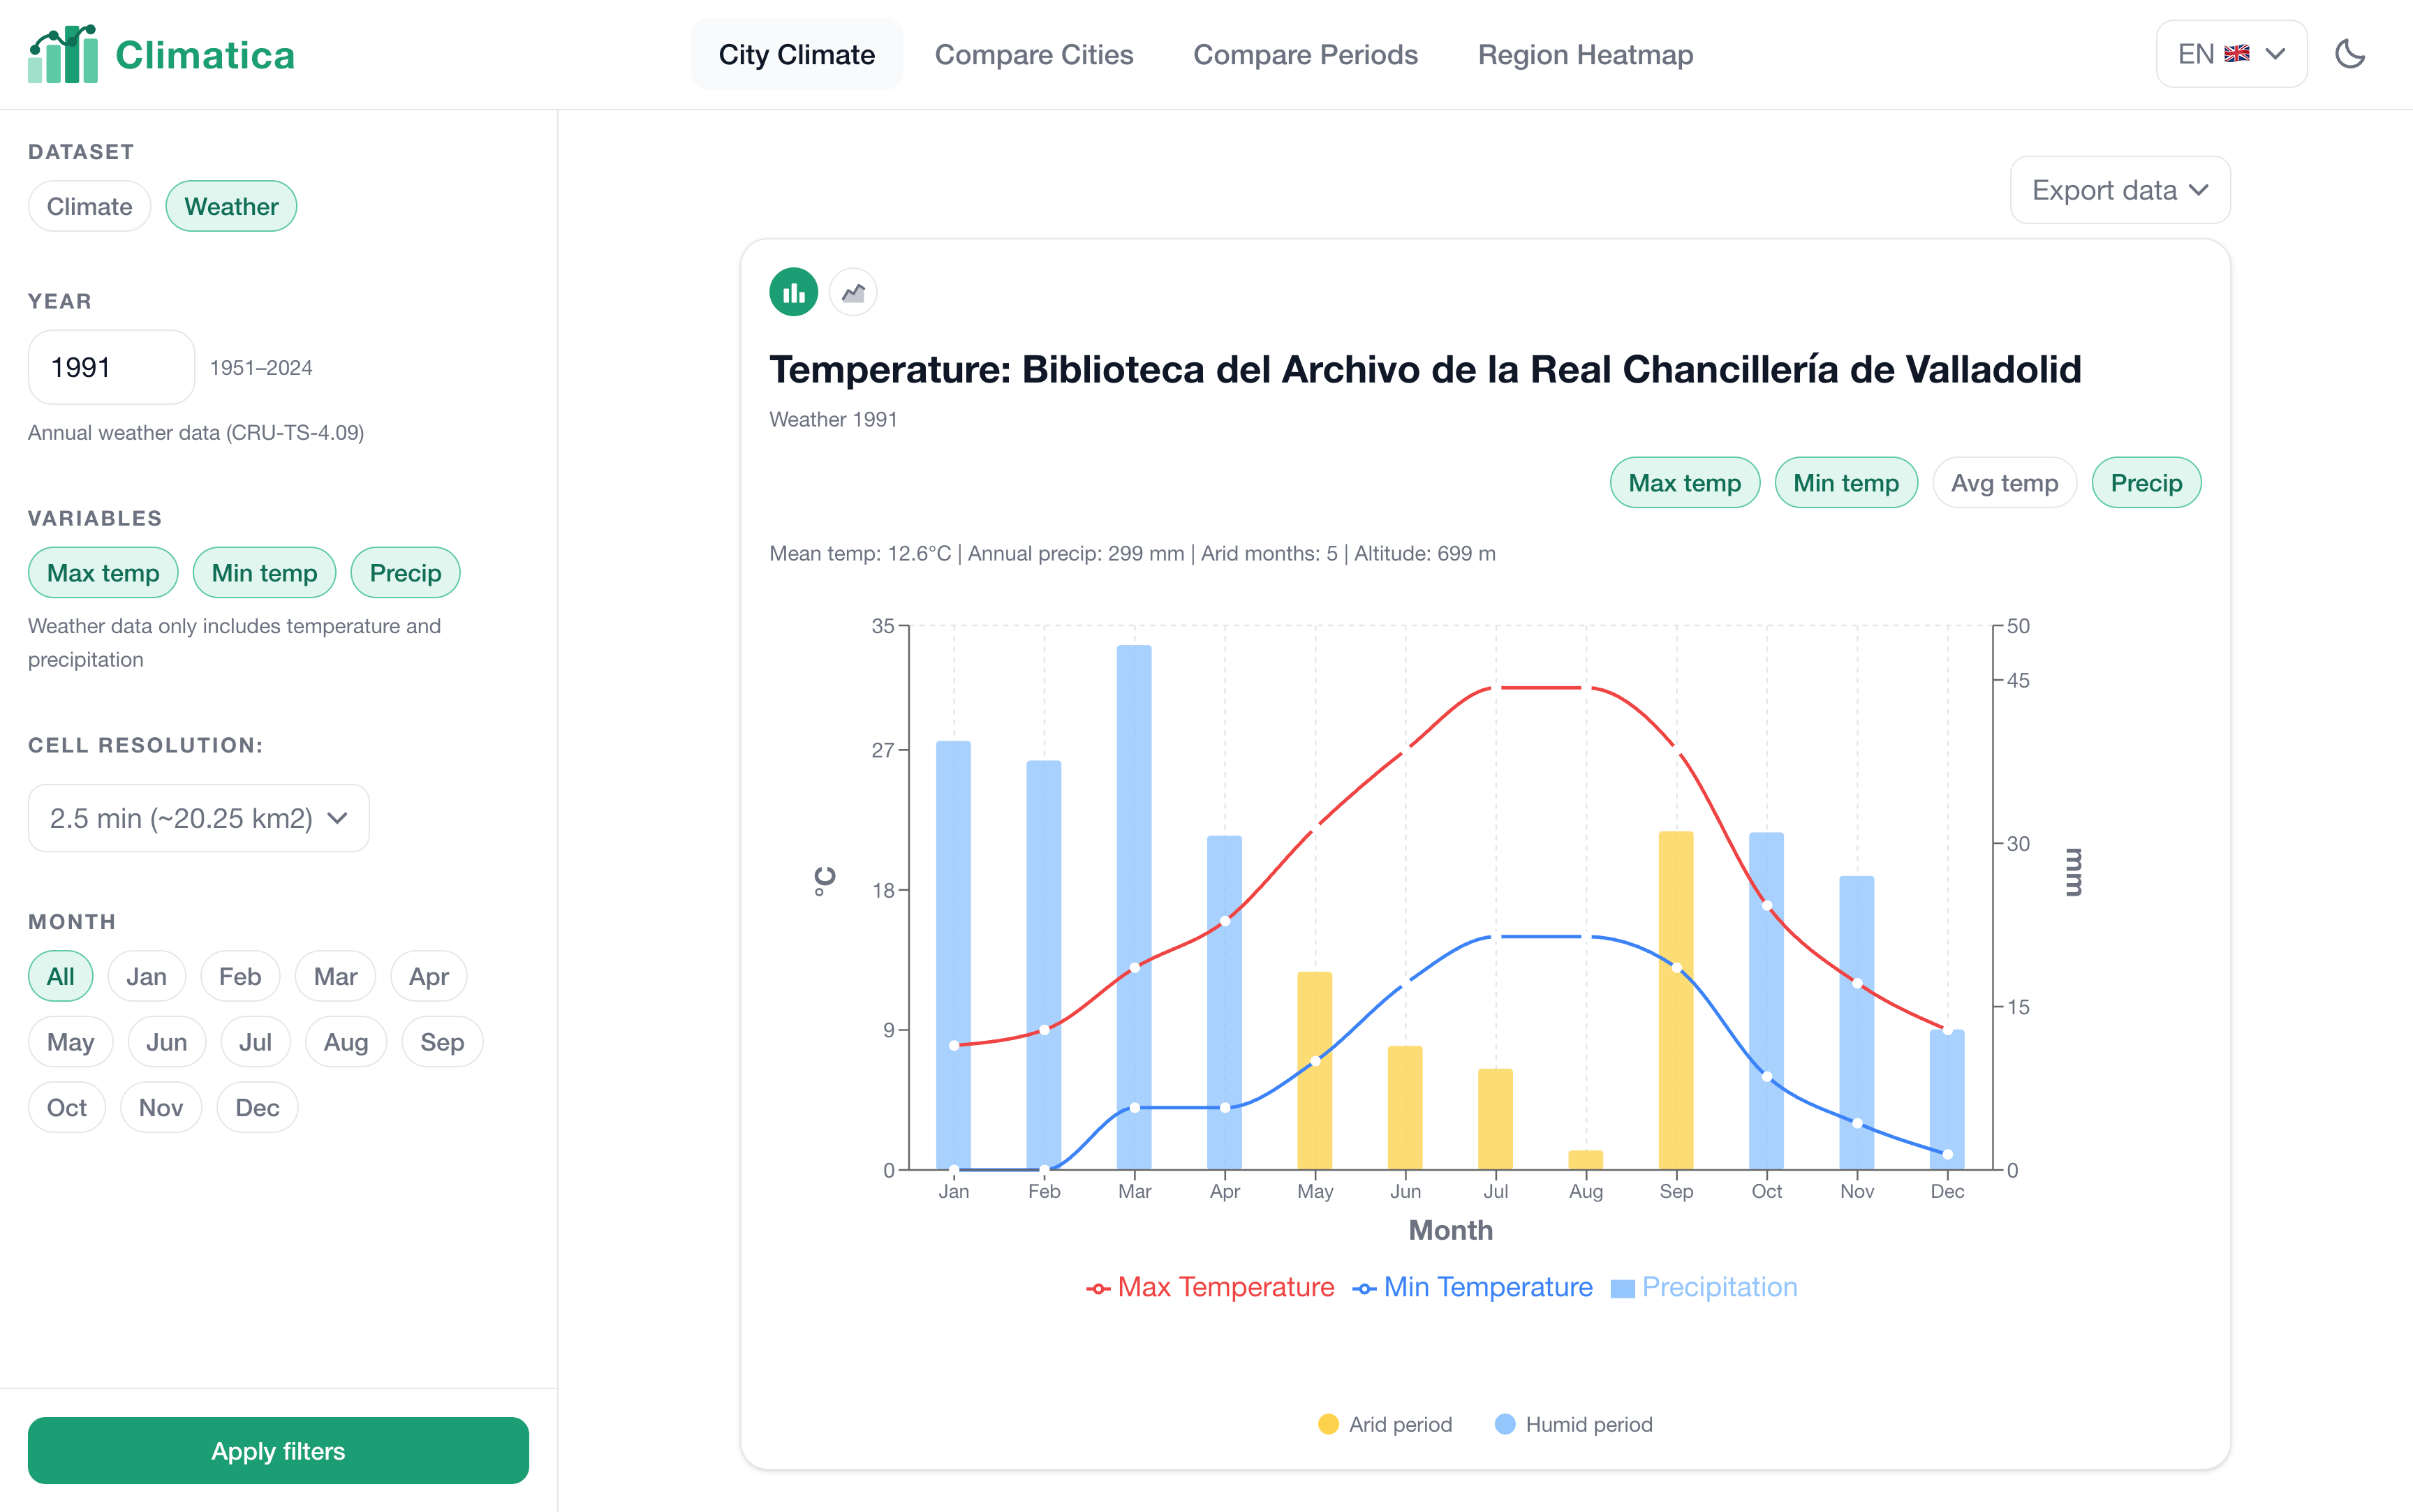
\includegraphics[width=0.9\textwidth]{Images/climatica-columns-graph.png}
  \caption{City Climate page --- standard climograph for Valladolid (weather
    dataset, year 1991). Precipitation is shown as bars; temperature as smooth
    lines. Blue bars indicate humid months; yellow bars indicate arid months.}
  \label{fig:page_city_std}
\end{figure}

\begin{figure}[t]
  \centering
  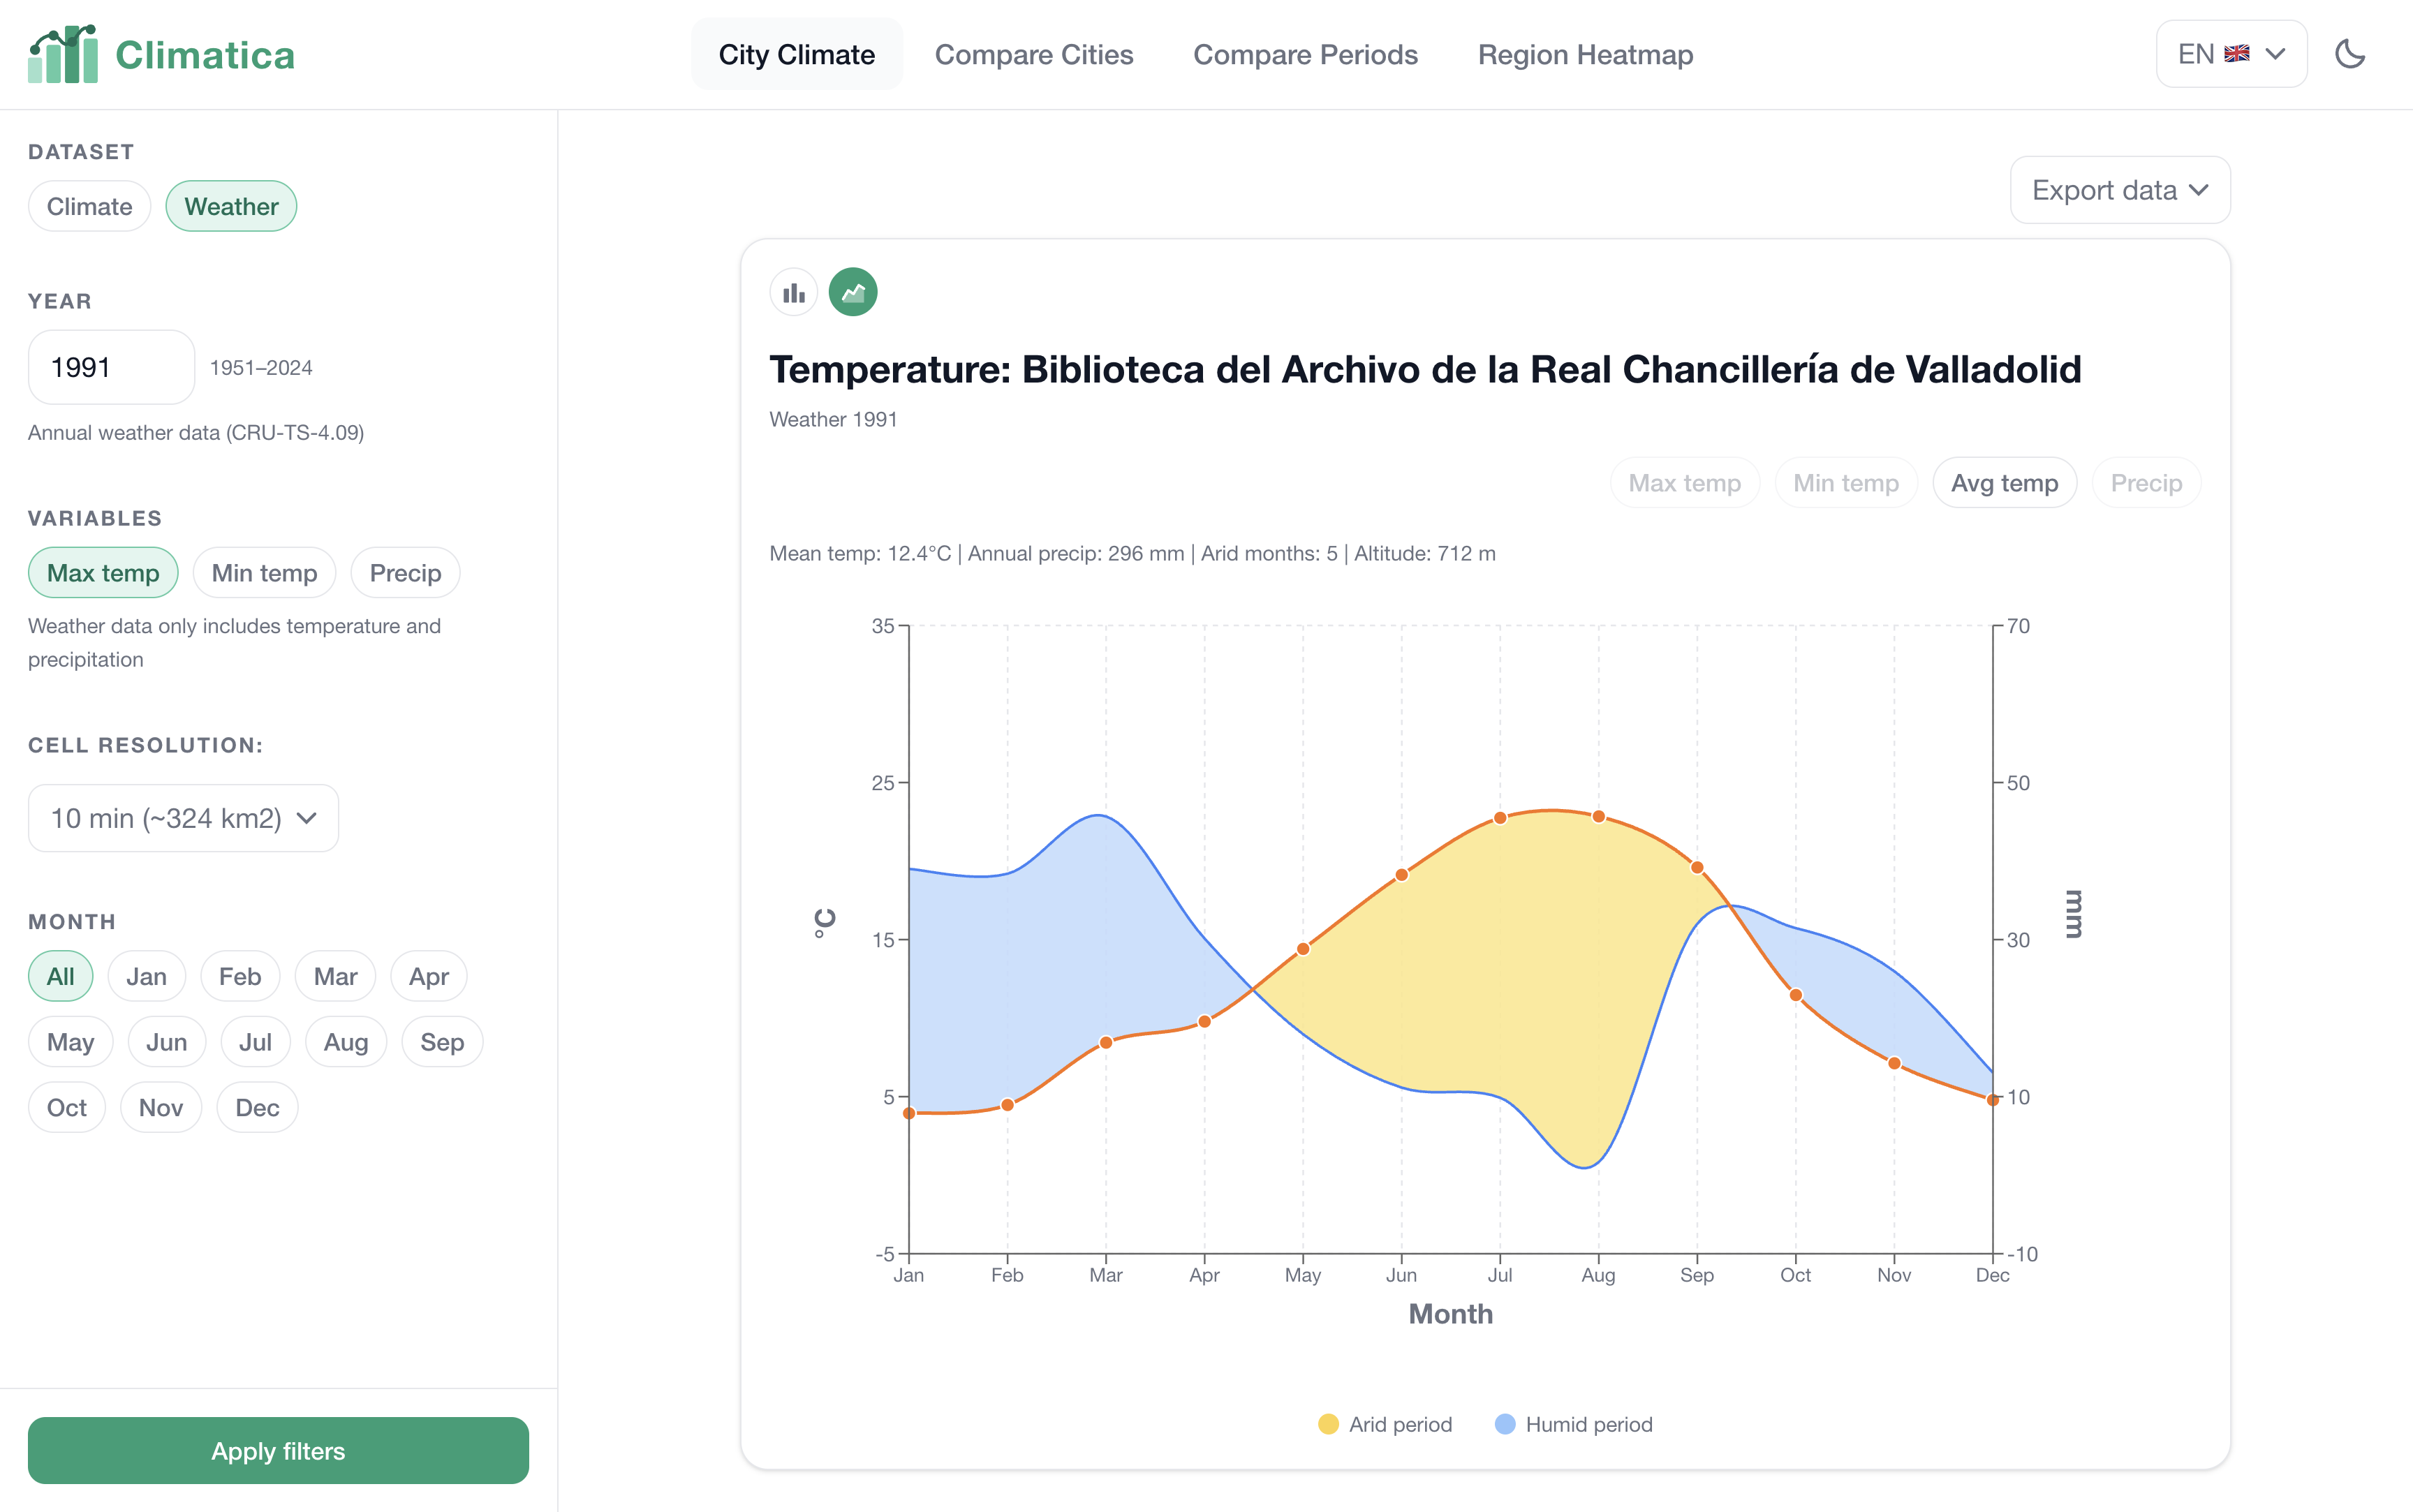
\includegraphics[width=0.9\textwidth]{Images/climatica-walter-lieth.png}
  \caption{City Climate page --- Walter-Lieth climatogram for the same city and
    period. Yellow filled areas indicate arid months; blue filled areas indicate
    humid months.}
  \label{fig:page_city_wl}
\end{figure}

Several technical details are worth noting. When the user clicks the map, a
provisional city object with the raw coordinates is committed to state
immediately so that the climate data fetch begins without waiting for Wikidata
reverse geocoding. If the geocoding call returns a named city, the label is
upgraded in place; a ref prevents stale responses from older clicks from
overwriting newer results. The raster cell outline is computed by parsing the
cell IRI returned by SCRAPI: the \texttt{\_r\{row\}c\{col\}} suffix encodes the
row and column indices, from which the bounding box is derived using the known
cell dimensions of the selected grid resolution.

\subsection{Compare Cities}\label{APP_PROTO_COMPARE}

The Compare Cities page (Figure~\ref{fig:page_compare}) allows the user to
select two cities --- identified by green (City~A) and orange (City~B) colour
codes --- and view their climate profiles overlaid on shared axes. The page
displays a colour-coded statistics table and four derived insight cards: warmer
city, city with more rainfall, hottest month, and coldest month. A mini-map in
the top-right corner shows the geographic positions of both cities.

\begin{figure}[t]
  \centering
  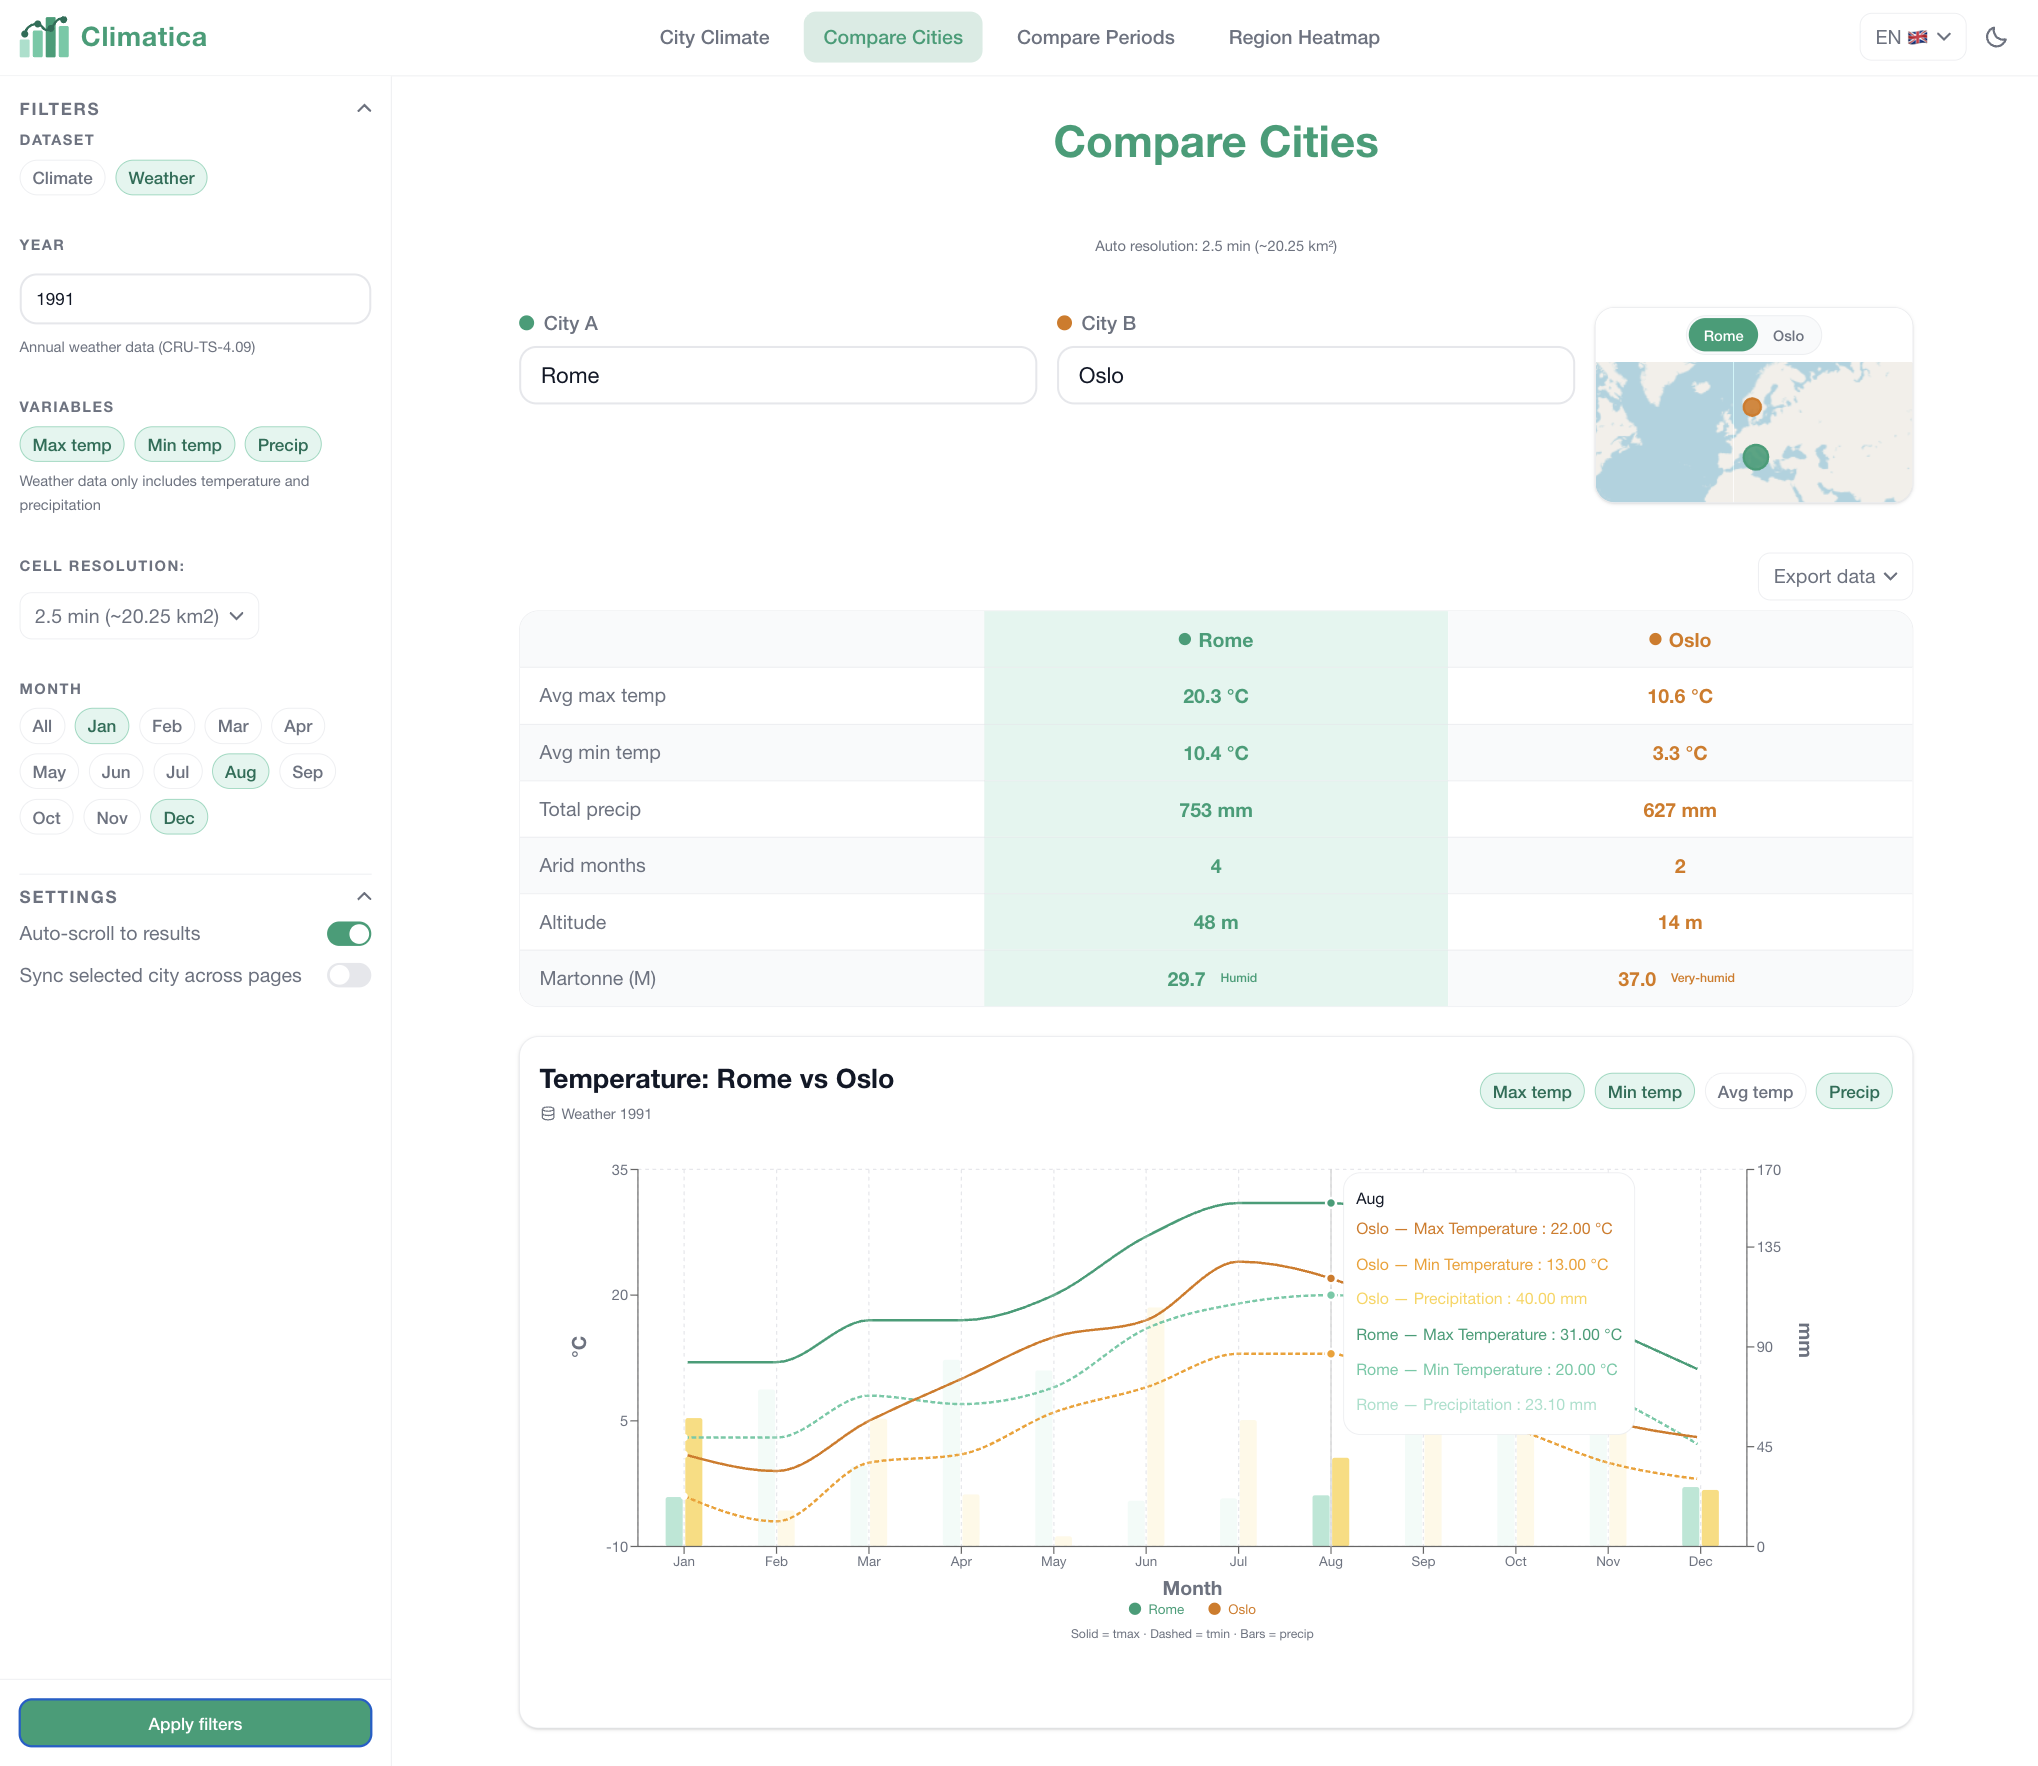
\includegraphics[width=0.9\textwidth]{Images/climatica-compare-cities.png}
  \caption{Compare Cities page comparing Rome and Oslo (weather dataset,
    year~1991). The upper section shows city search fields, a mini-map, and a
    colour-coded statistics table; the lower section shows the overlaid
    temperature and precipitation chart with derived insight cards.}
  \label{fig:page_compare}
\end{figure}

Both cities are fetched in parallel using \texttt{Promise.all} inside a single
TanStack Query entry. City selections are written to URL search parameters,
enabling the comparison to be shared by copying the URL.

\subsection{Compare Periods}\label{APP_PROTO_PERIODS}

The Compare Periods page allows the user to analyse how the climate of a single
city has shifted across time. The page operates in two distinct modes depending
on the active dataset.

\textbf{Climate mode} (Figure~\ref{fig:page_periods_climate}) compares exactly
two 30-year climate normals chosen from the five available periods
(1951--1980, 1961--1990, 1970--2000, 1981--2010, 1991--2020). The two periods
are selected via dropdowns and their monthly data are fetched in parallel via
\texttt{Promise.all} with \texttt{keepPreviousData: true}, so the chart remains
visible while new data loads. Below the overlaid chart, two trend indicator
cards summarise the change: one for maximum temperature and one for total
precipitation. Positive differences are coloured with the Period~B accent colour
and negative differences with Period~A, giving an immediate visual indication of
warming or drying trends.

\textbf{Weather mode} (Figure~\ref{fig:page_periods_weather}) supports between
2 and 5 individual years selected from the CRU-TS-4.09 archive (1951--2024).
Years are managed through the sidebar filter panel (Figure~\ref{fig:page_periods_sidebar})
and persisted to \texttt{localStorage} via a Zustand store. Each selected year
is fetched as a separate parallel TanStack Query (\texttt{useQueries}), and
results accumulate progressively as they arrive --- columns for still-loading
years show skeleton placeholders in the statistics table, making partial results
immediately visible without blocking the entire view. Each year is assigned one
of five fixed colours (green~$\to$~amber~$\to$~blue~$\to$~rose~$\to$~violet),
all overlaid on a single shared chart.

\begin{figure}[t]
  \centering
  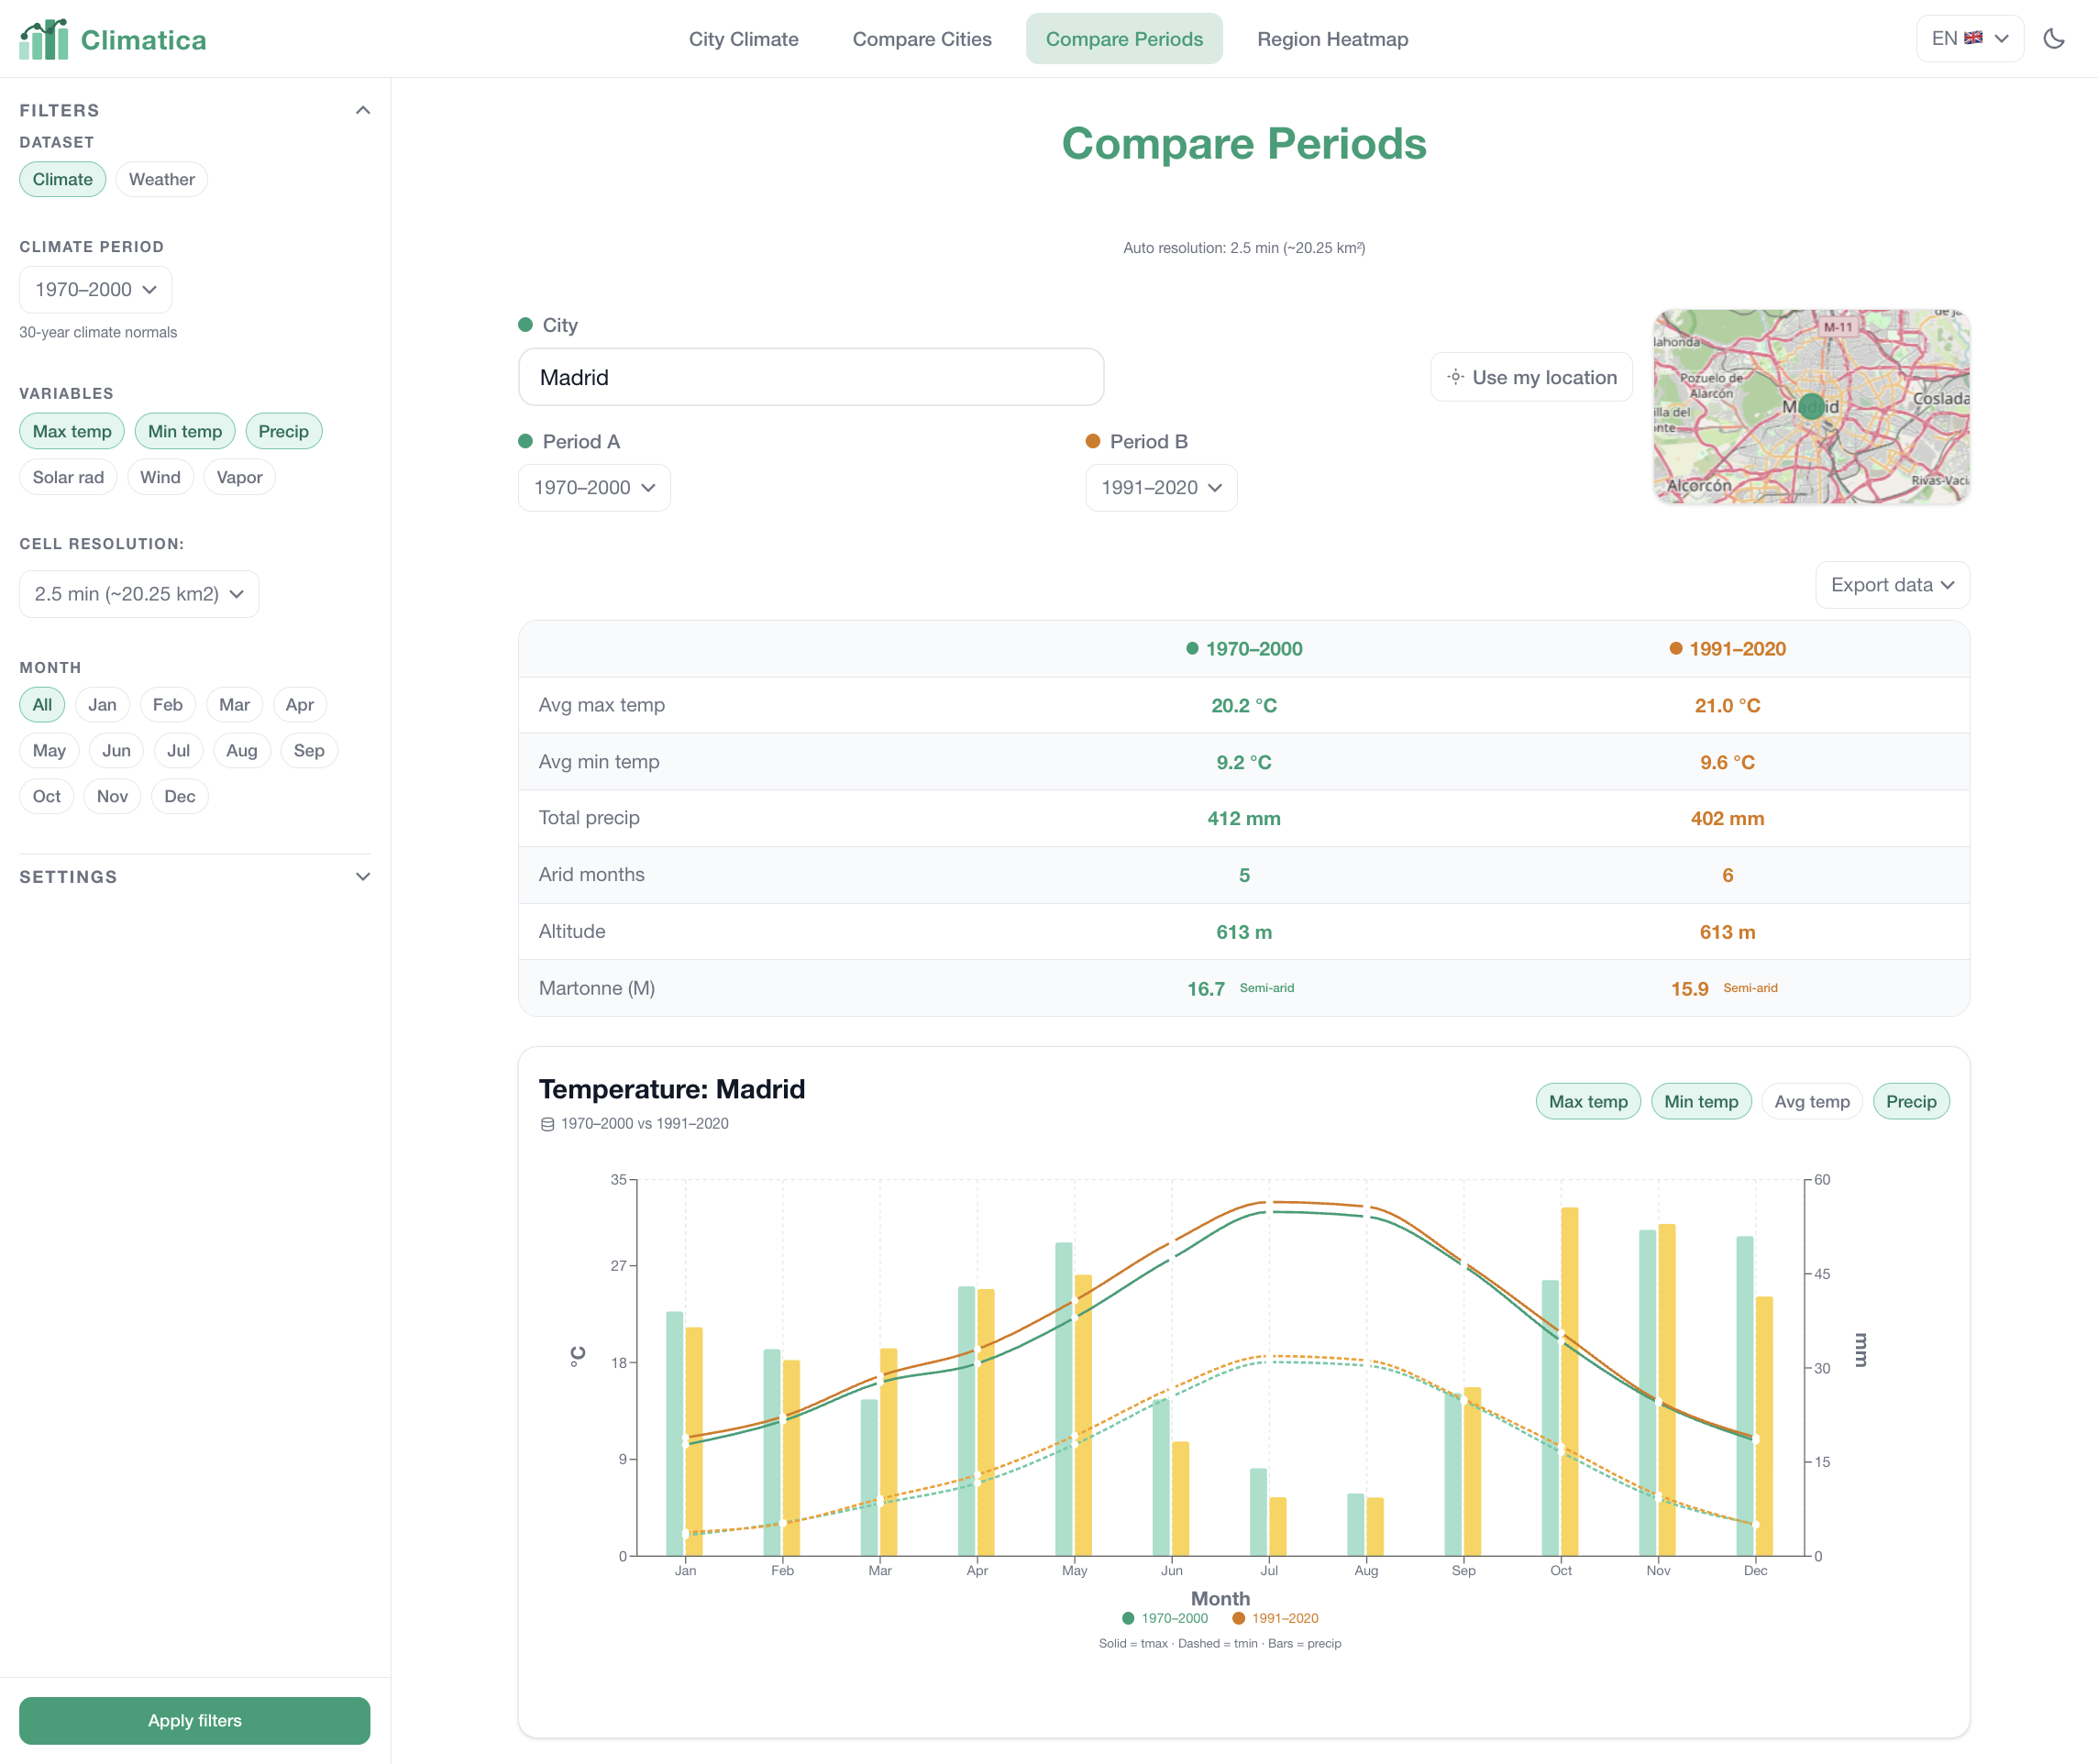
\includegraphics[width=0.9\textwidth]{Images/climatica-compare-periods-climate.png}
  \caption{Compare Periods page --- climate mode for Madrid, comparing the
    1970--2000 and 1991--2020 climate normals. The statistics table shows a
    warming trend (+0.8\,°C avg max) and slight decrease in precipitation
    between the two periods.}
  \label{fig:page_periods_climate}
\end{figure}

\begin{figure}[t]
  \centering
  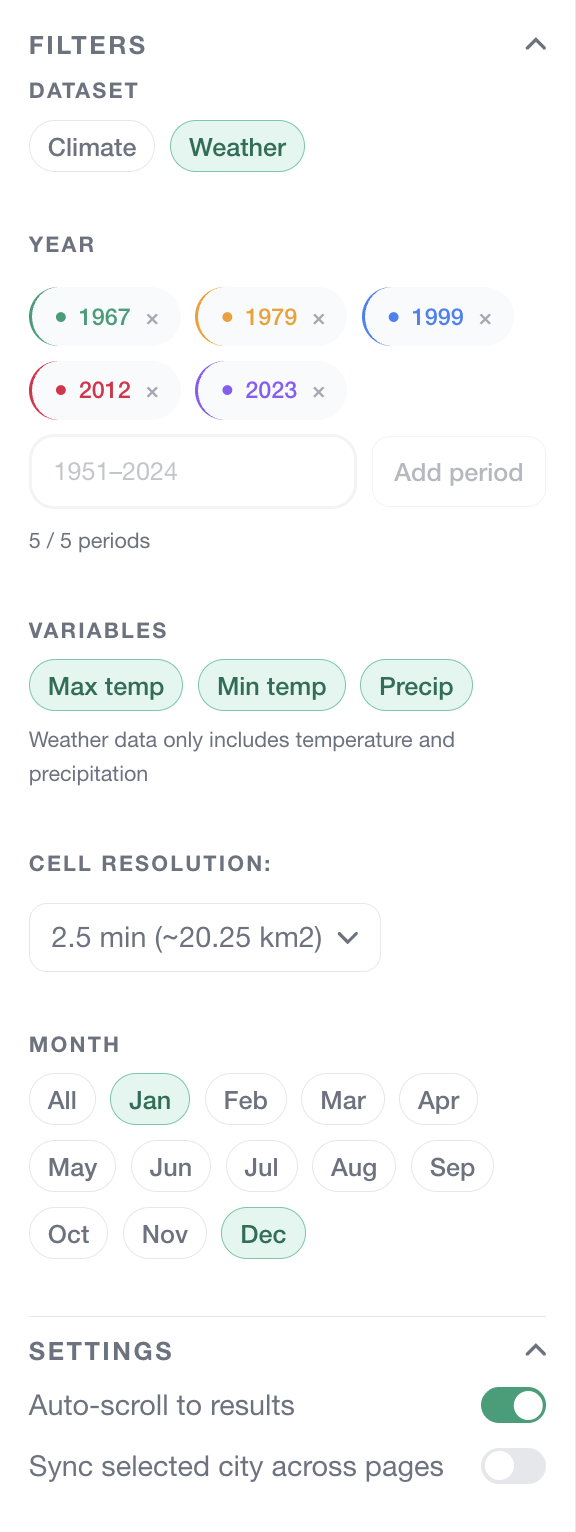
\includegraphics[width=0.5\textwidth]{Images/climatica-compare-periods-sidebar.png}
  \caption{Compare Periods page --- sidebar in weather mode with five years
    selected (1967, 1979, 1999, 2012, 2023). Each year receives a distinct
    colour that carries through to the chart and statistics table. The
    \emph{Add period} input allows adding years up to the maximum of five.
    The Settings section exposes the auto-scroll and city sync toggles.}
  \label{fig:page_periods_sidebar}
\end{figure}

\begin{figure}[t]
  \centering
  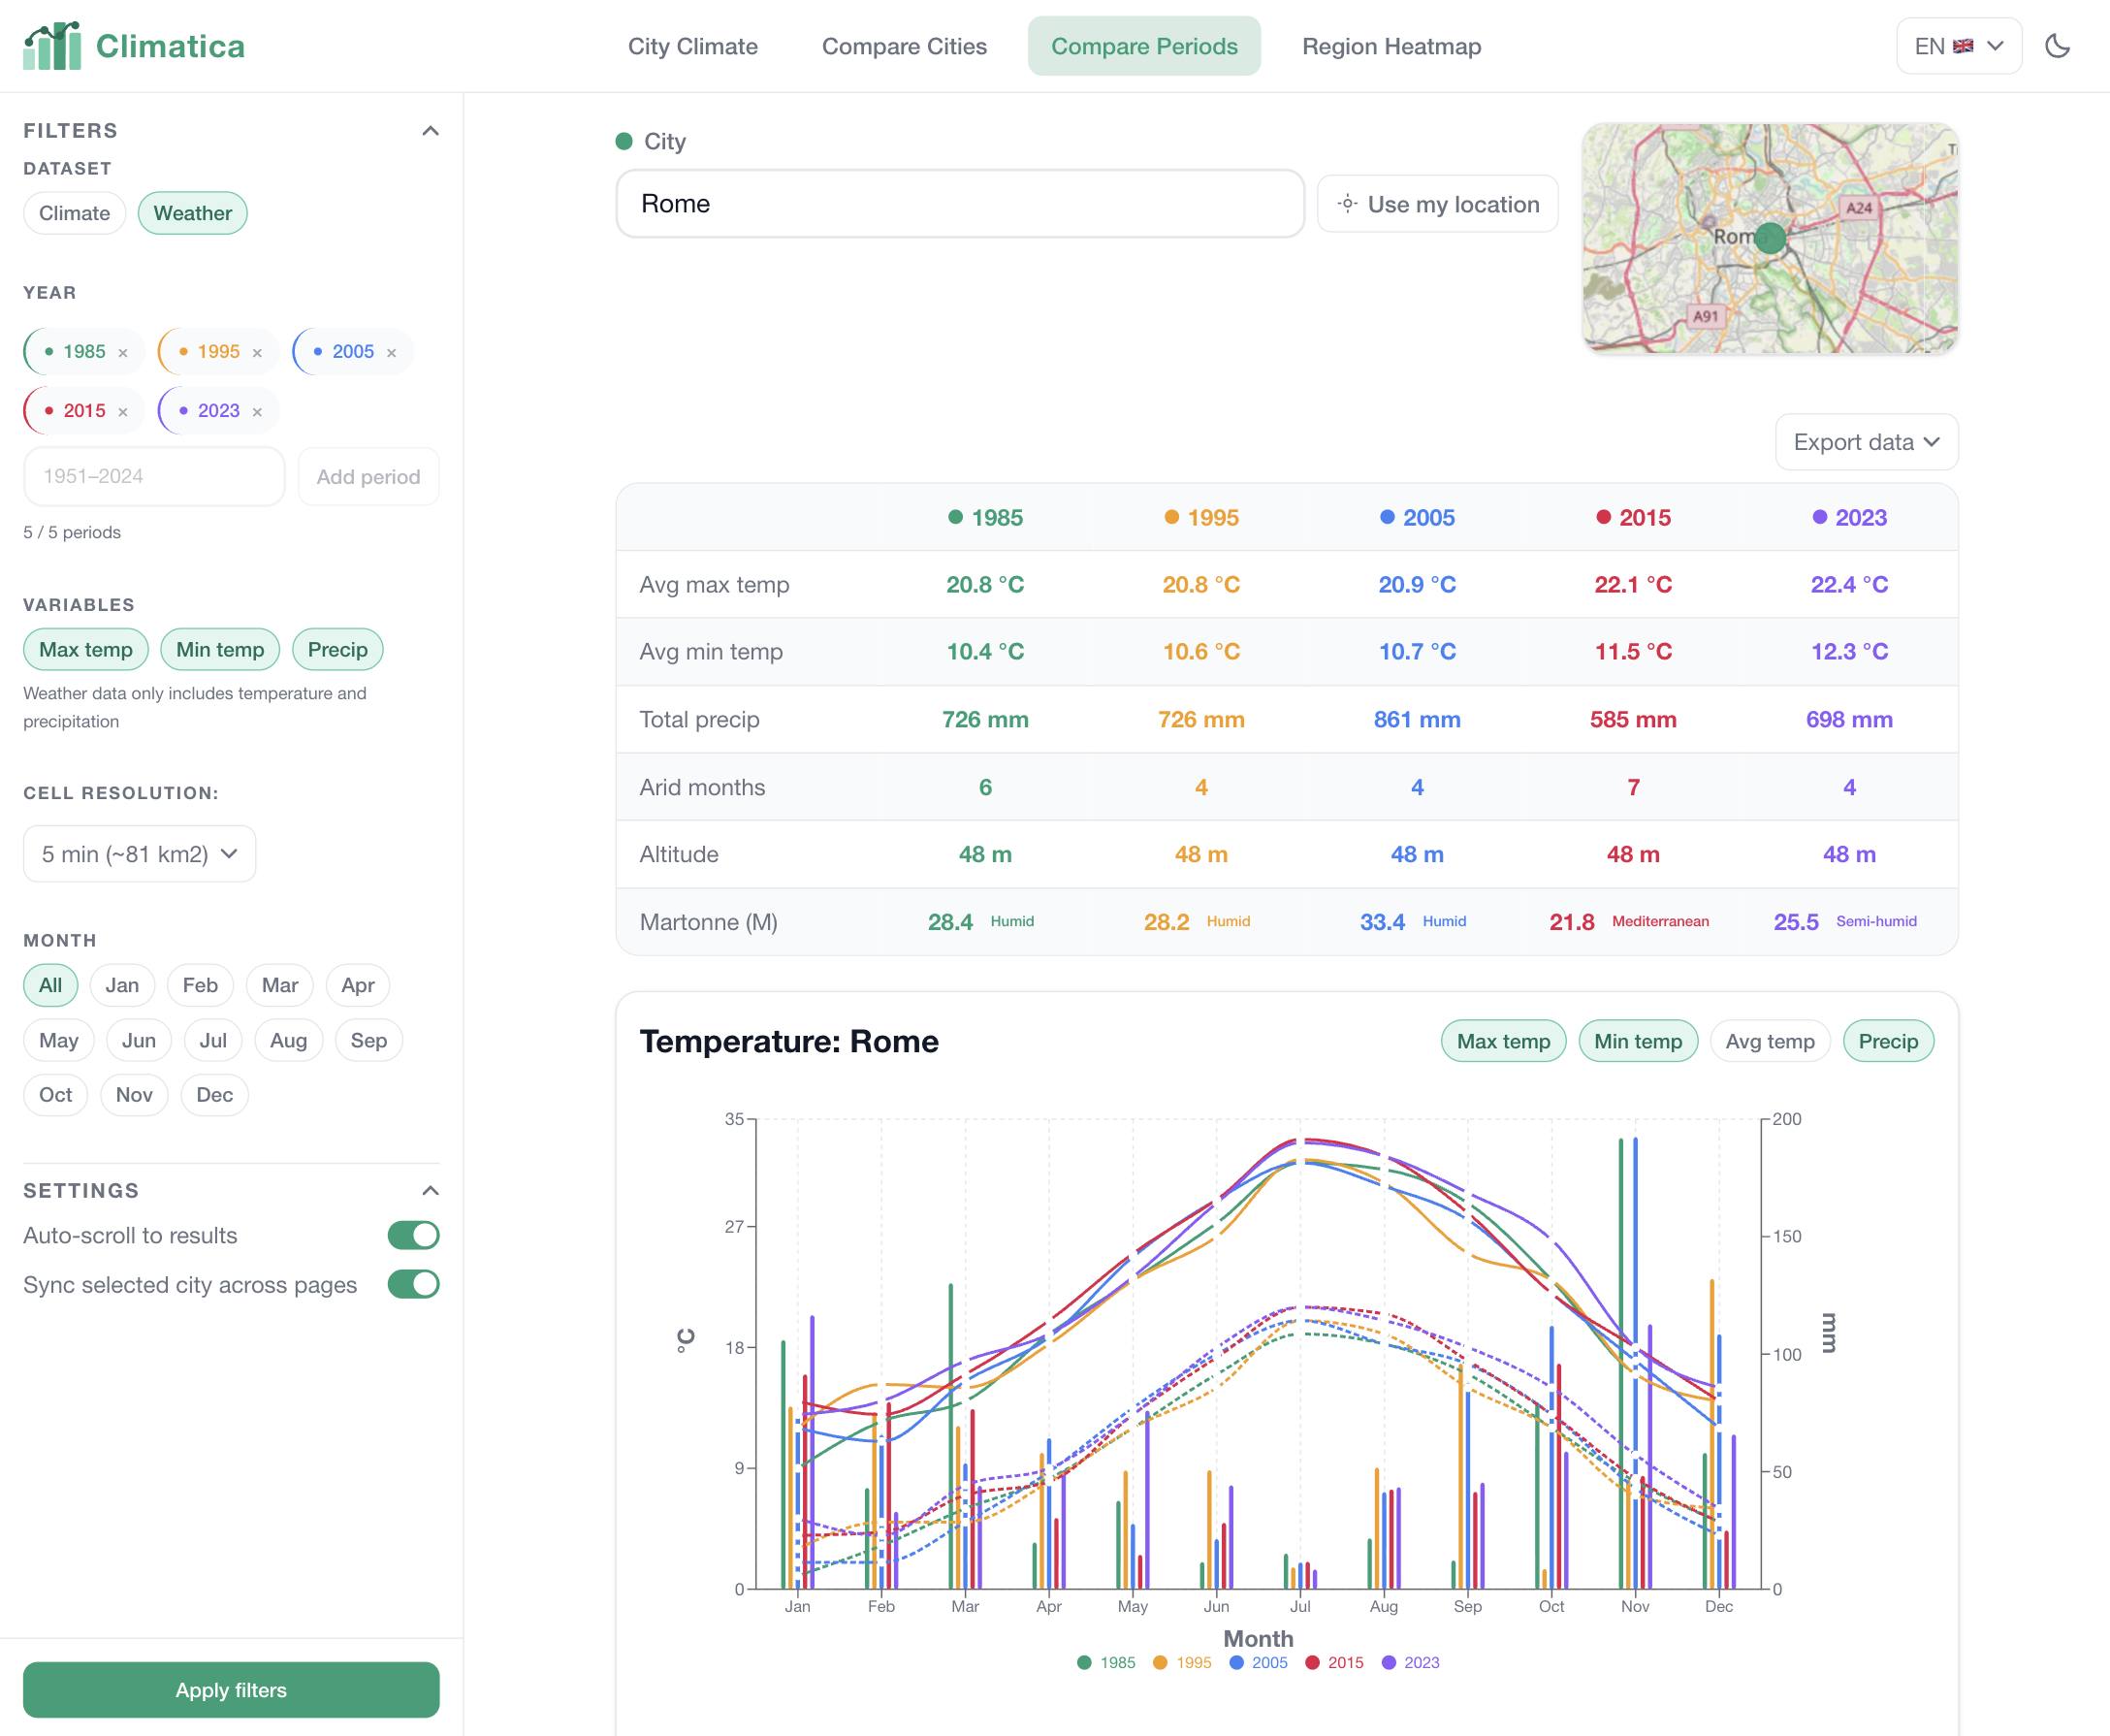
\includegraphics[width=0.9\textwidth]{Images/climatica-compare-periods-weather.png}
  \caption{Compare Periods page --- weather mode with multiple years selected
    simultaneously. Each year is rendered in a distinct colour; the statistics
    table shows one column per year with skeleton placeholders for years still
    loading.}
  \label{fig:page_periods_weather}
\end{figure}

\subsection{Region Heatmap}\label{APP_PROTO_HEATMAP}

The Region Heatmap page allows the user to analyse the spatial distribution of
a climate variable across a geographic region. The user selects a drawing mode
--- bounding box or freeform polygon --- and draws directly on the Leaflet map.
The application then queries all WorldClim raster pixels within the selection
and renders each pixel as a coloured rectangle, forming a spatially resolved
heatmap.

\textbf{Selection modes.} The drawing mode is represented as a discriminated
type with three states: \texttt{"none"}, \texttt{"bbox"}, and
\texttt{"polygon"}. Only one mode is active at a time; switching clears the
opposite selection. The bounding box drawer disables map dragging during
interaction and commits the selection on mouse up. The polygon drawer
accumulates vertices on click; when three or more vertices exist and the cursor
comes within 14 pixels of the first vertex, a snap indicator appears and the
next click closes the polygon. Both selections are persisted in URL search
parameters for shareability.

\textbf{Data fetching.} Two hooks handle the two selection modes:
\texttt{useGetHeatmapData} for bounding boxes and
\texttt{useGetHeatmapPolygonData} for polygons. Each hook fires a single
TanStack Query whose \texttt{queryFn} issues two SCRAPI requests in a
\texttt{Promise.all}: one for the per-pixel grid and one for the area-average
summary shown in the regional profile panel. The inactive hook is disabled
automatically because its input is \texttt{null}.

\textbf{Pixel rendering.} Pixels are rendered as rectangle overlays on the
Leaflet map, managed by a single \texttt{L.layerGroup}. Each \texttt{L.rectangle}
is a Leaflet primitive that accepts geographic bounds and renders as a coloured
tile on the map canvas. On every relevant state change, the group is cleared
and rebuilt. The geographic position of each rectangle is computed from the
pixel IRI returned by SCRAPI: the \texttt{\_r\{row\}c\{col\}} suffix is parsed
to recover the row and column index, from which the cell bounding box is derived
as $\mathit{north} = 90 - \mathit{row} \times \mathit{cellSize}$ and
$\mathit{west} = -180 + \mathit{col} \times \mathit{cellSize}$. This avoids
any dependency on explicit latitude/longitude fields, which are absent for
water cells.

\textbf{Colour scale.} The normalisation formula is
$t = (\mathit{value} - \mathit{min}) / (\mathit{max} - \mathit{min})$, where
\textit{min} and \textit{max} are the observed extremes in the current response.
Two palettes are available: a nine-stop RdYlBu diverging palette for temperature
(blue cold $\to$ red hot) and a four-stop sequential brown palette for
precipitation. The legend bar samples the colour function at ten evenly spaced
positions and renders a CSS \texttt{linear-gradient}.

Figures~\ref{fig:page_heatmap_bbox} and~\ref{fig:page_heatmap_polygon} show
the heatmap page in bounding box and polygon selection modes respectively.
\begin{figure}[t]
  \centering
  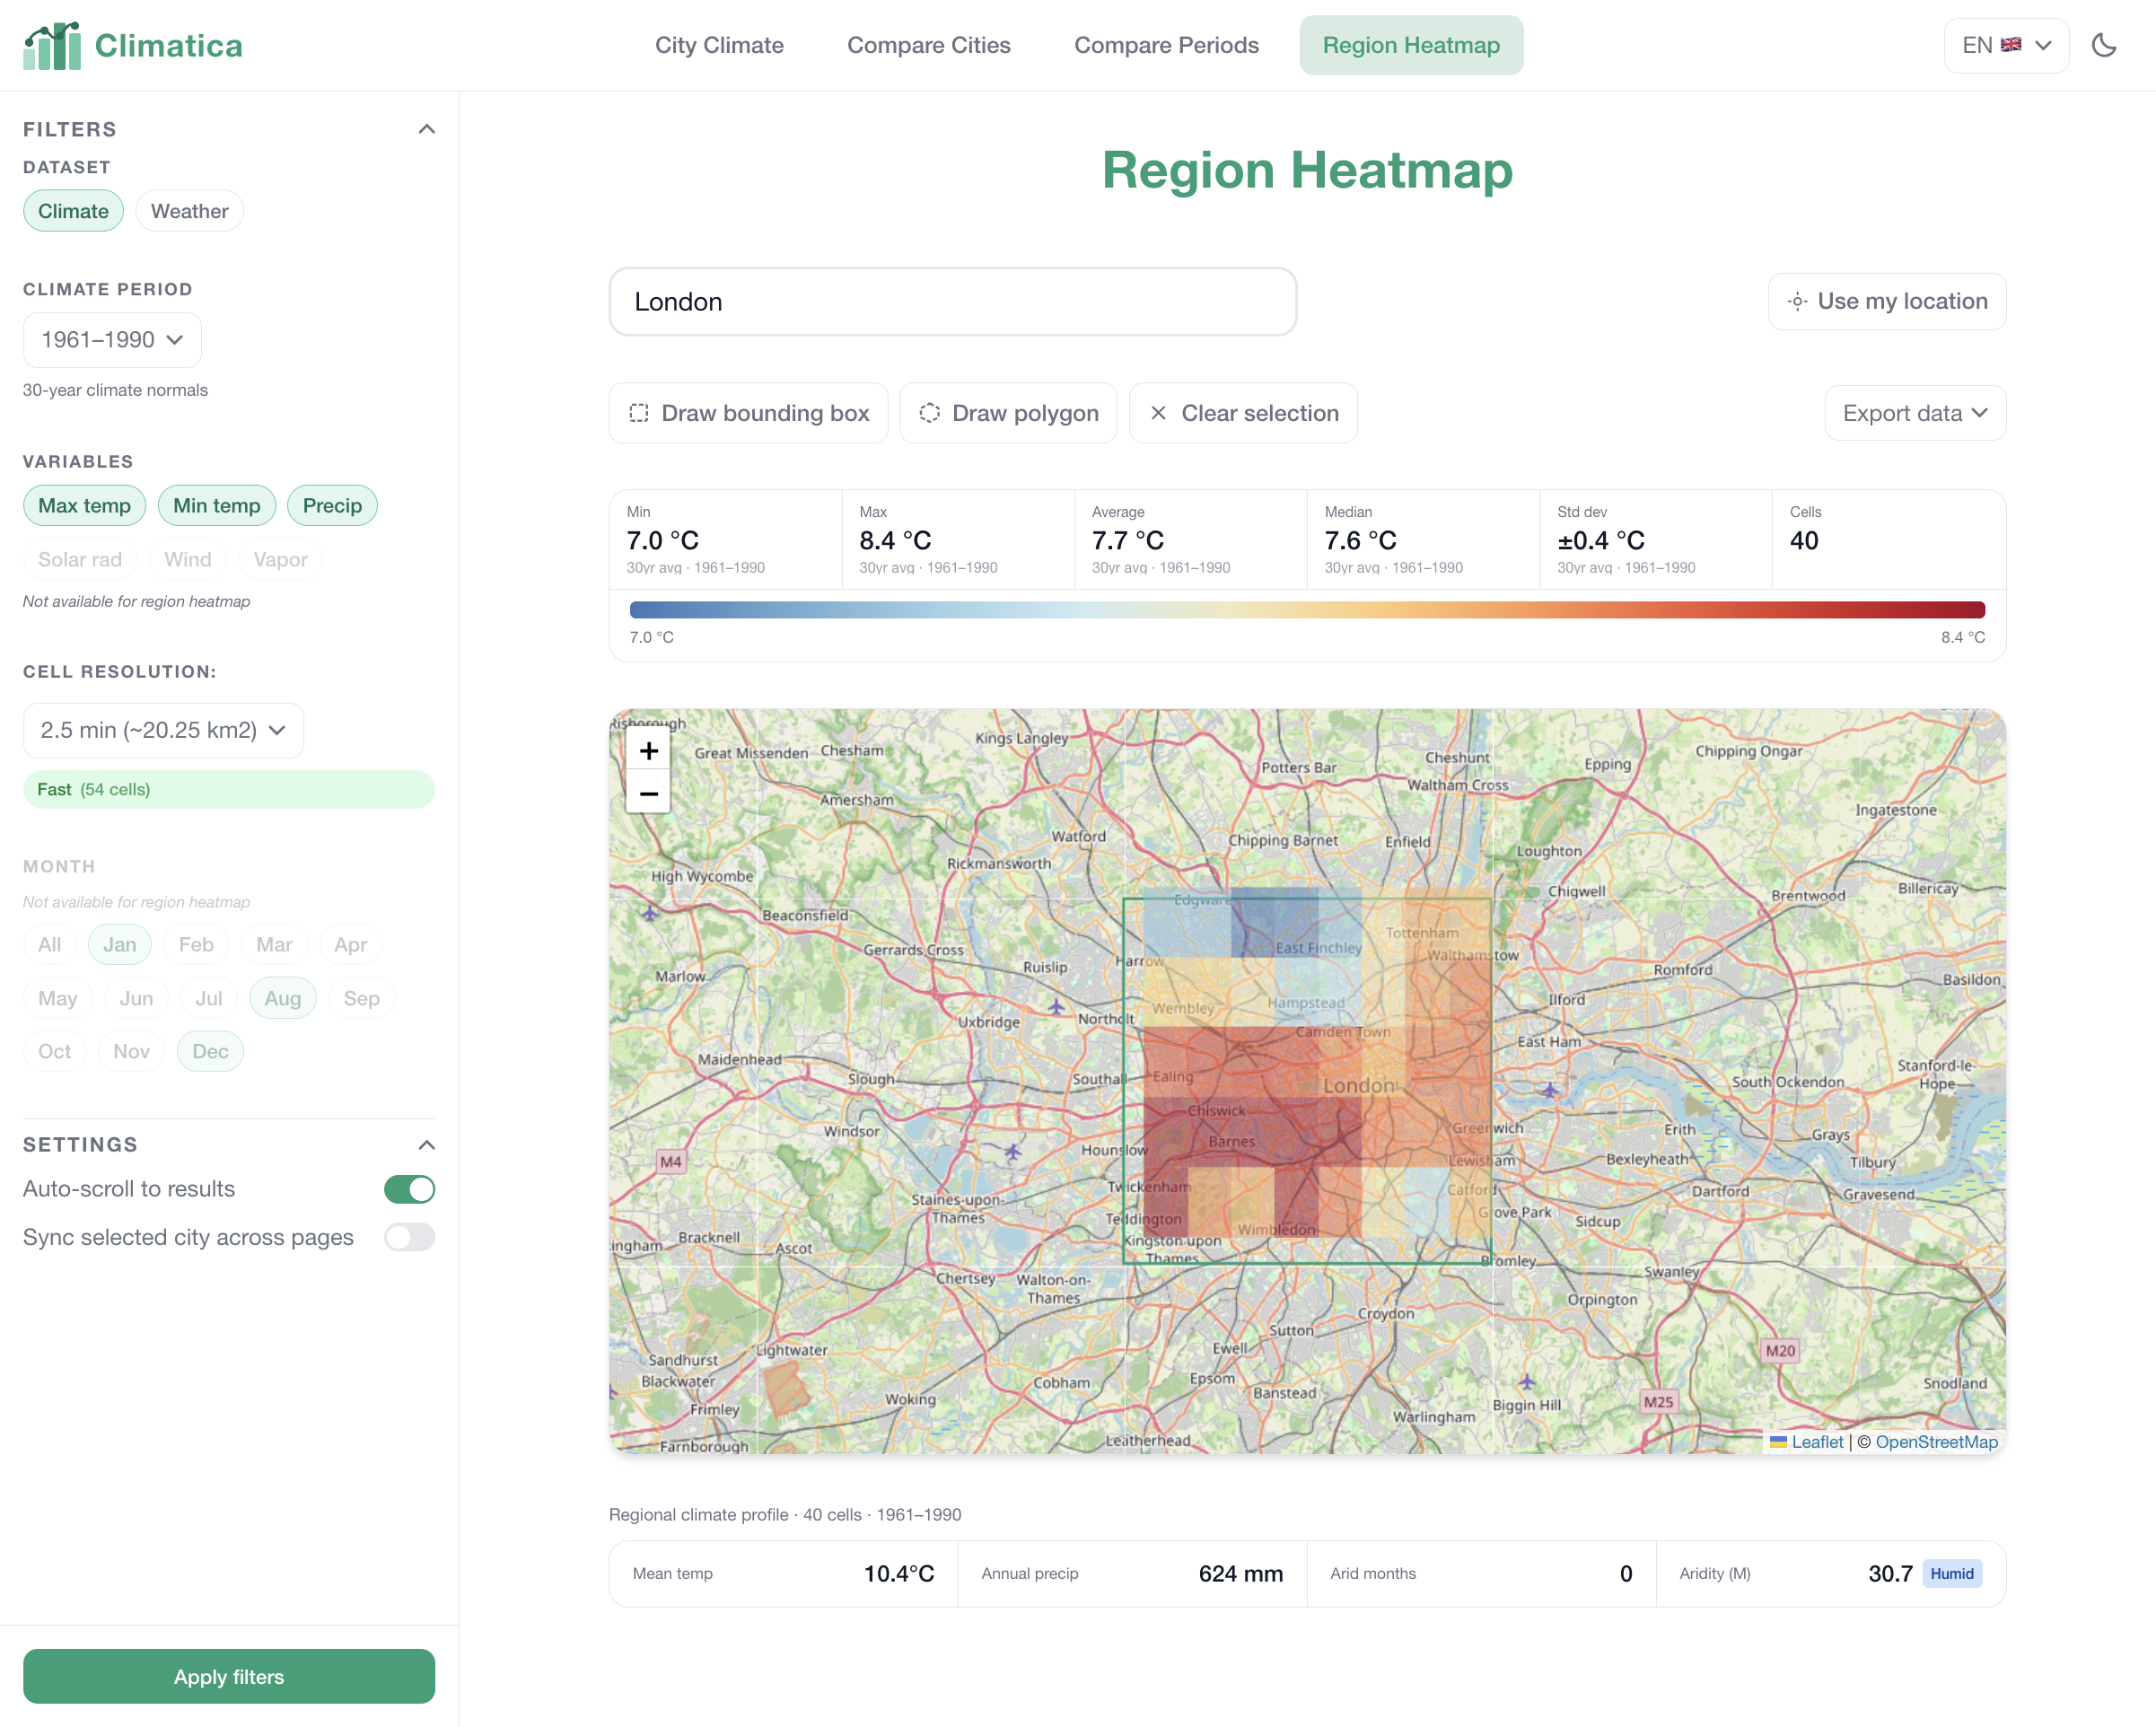
\includegraphics[width=0.9\textwidth]{Images/climatica-heatmap-bbox.png}
  \caption{Region Heatmap page --- bounding box selection over Greater London
    (climate dataset, 1961--1990, maximum temperature). The colour scale runs
    from blue (7.0\,°C) to red (8.4\,°C); the regional profile below the map
    summarises the 40 queried cells with mean temperature, annual precipitation,
    arid months, and the Martonne aridity index.}
  \label{fig:page_heatmap_bbox}
\end{figure}

\begin{figure}[t]
  \centering
  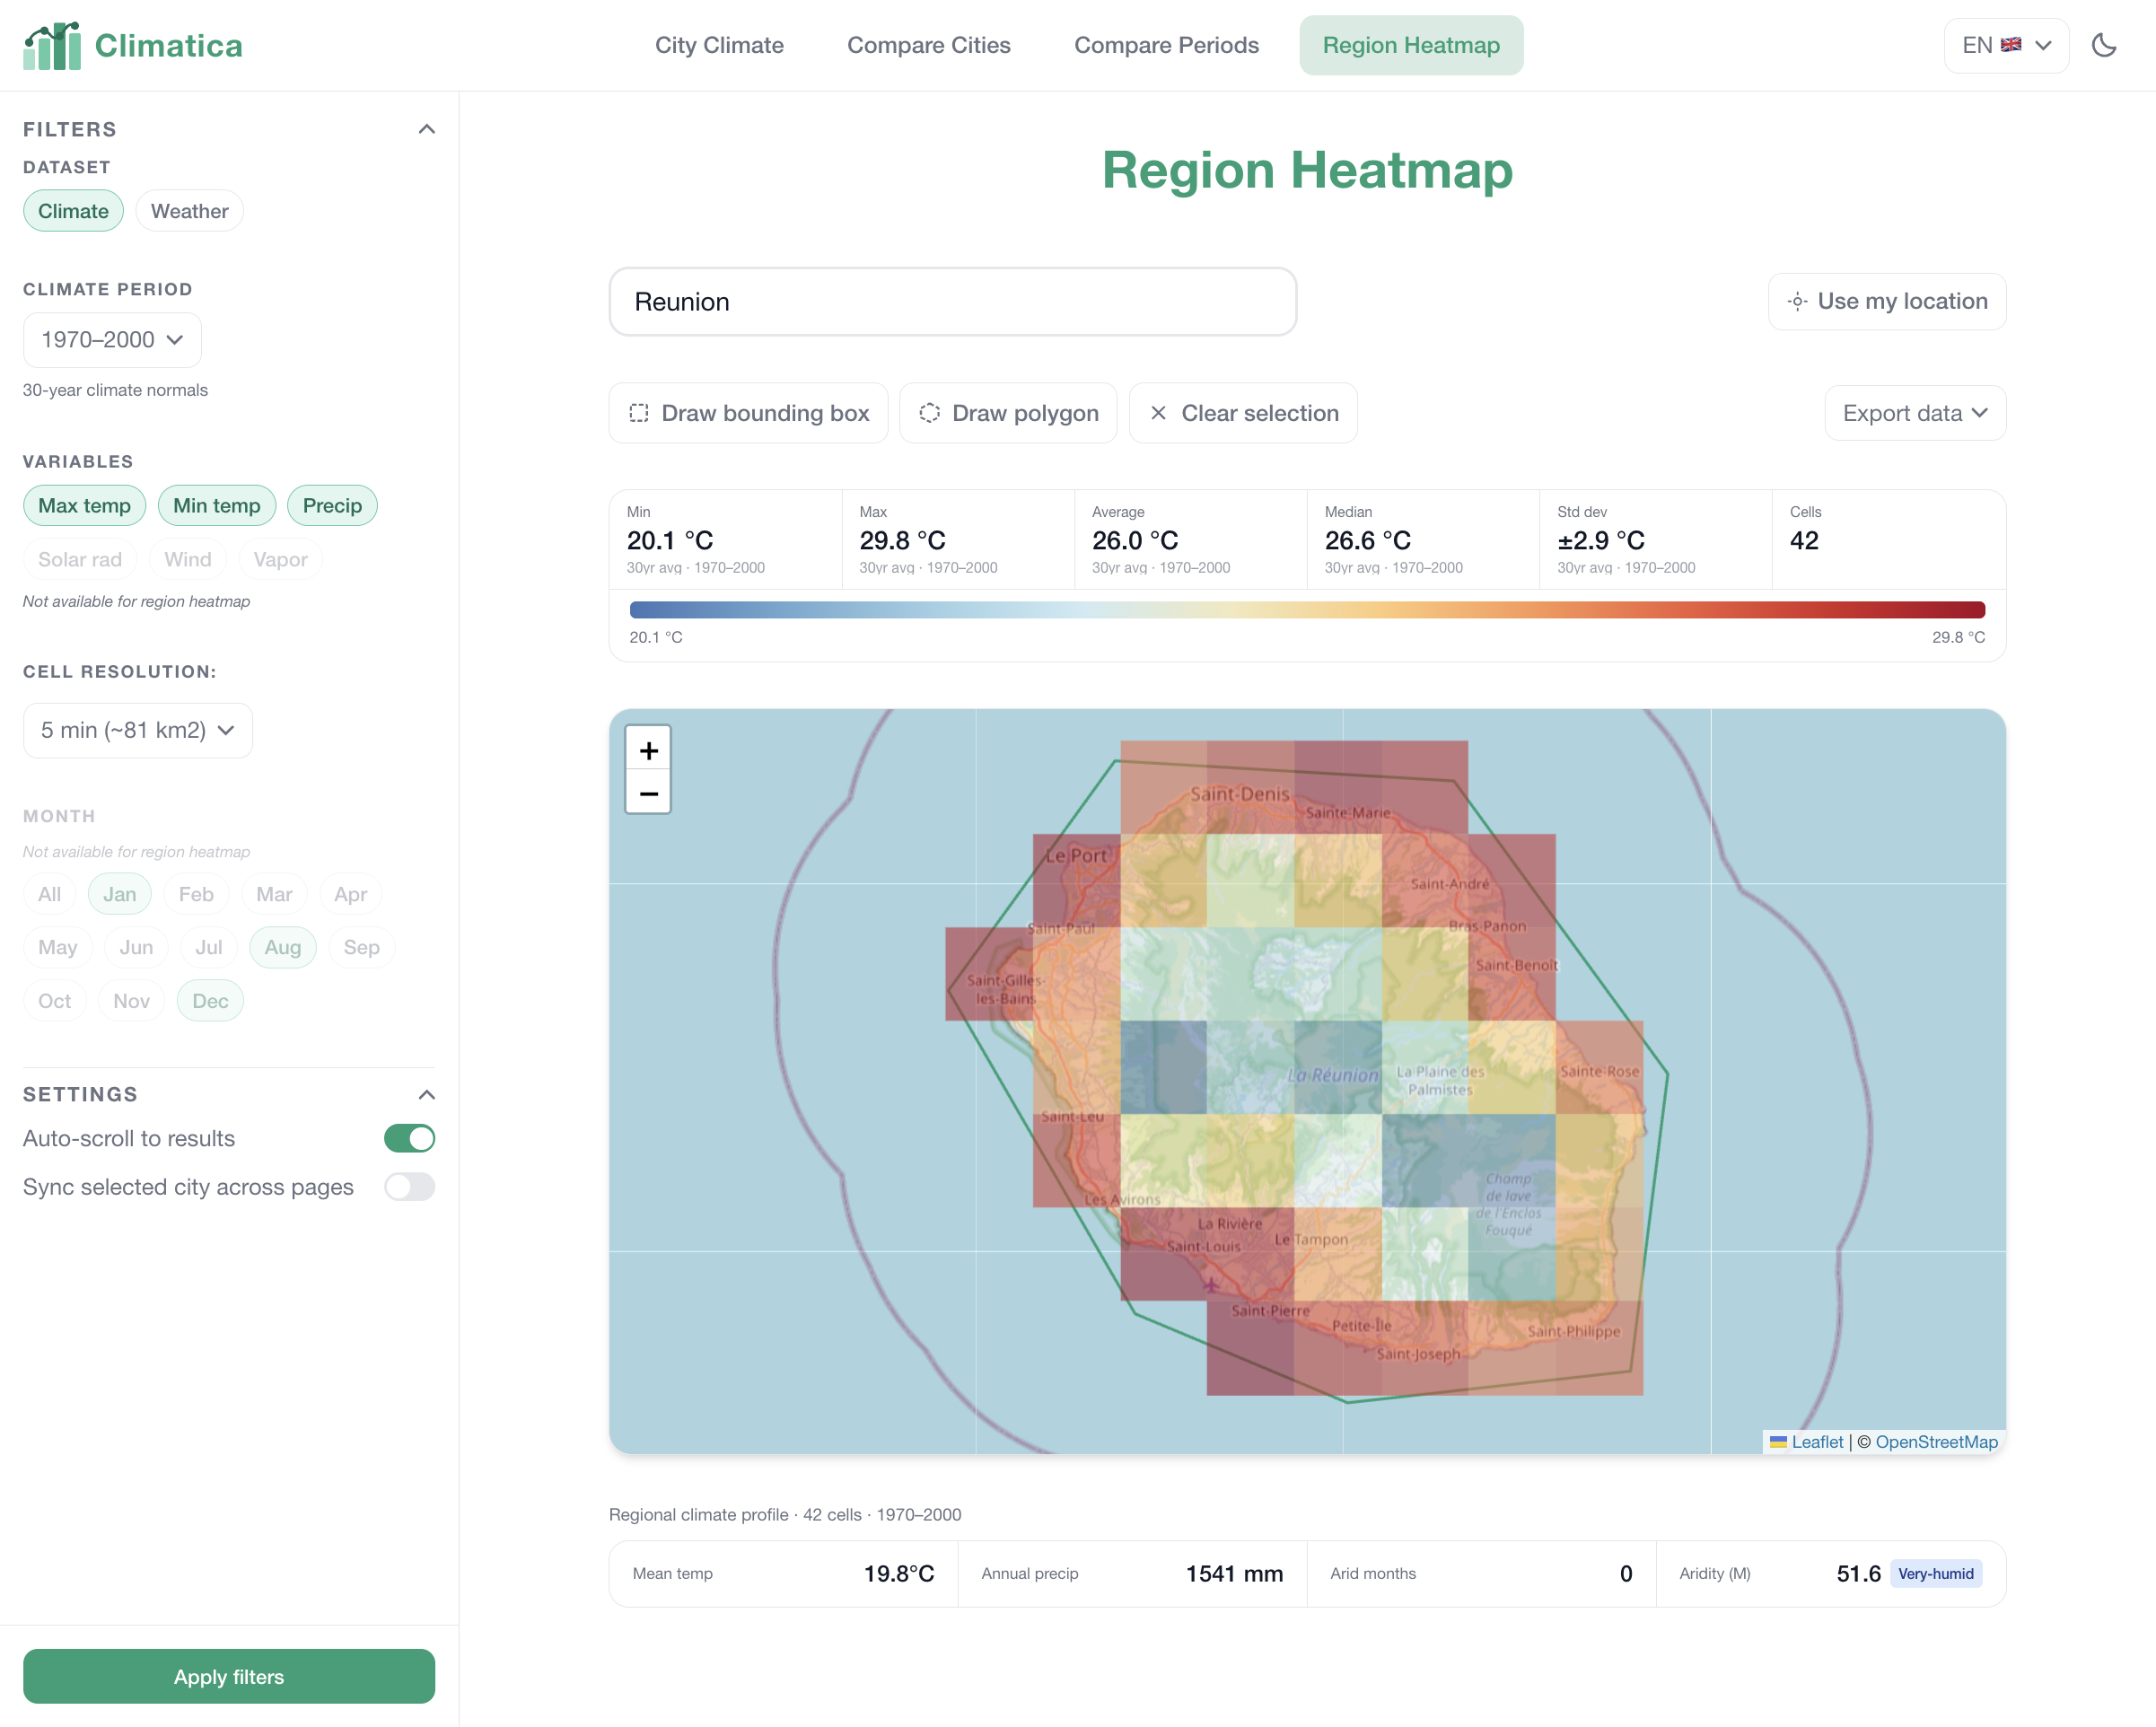
\includegraphics[width=0.9\textwidth]{Images/climatica-heatmap-polygon.png}
  \caption{Region Heatmap page --- freeform polygon selection over the island
    of Réunion (climate dataset, 1970--2000, maximum temperature). The polygon
    boundary is drawn by the user vertex by vertex; the application queries all
    42 raster cells whose centroids fall within the polygon. The wide
    temperature range (20.1--29.8\,°C) reflects the island's significant
    elevation gradient from coastal lowlands to the volcanic highlands.}
  \label{fig:page_heatmap_polygon}
\end{figure}

\textbf{Known limitation: longitude wraparound.} Leaflet allows the user to
pan the map indefinitely eastward, producing longitudes greater than 180°
(e.g.\ 355°). SCRAPI does not accept out-of-range longitudes, so queries
issued from such positions return no data. A fix would normalise the longitude
to the range $[-180, 180]$ before issuing the SCRAPI request; this is left as
future work.

\subsection{Accessing the Application}\label{APP_PROTO_ACCESS}

Climatica is publicly accessible at \url{https://climatica.gsic.uva.es/}.
The application runs entirely in the browser and requires no installation or
registration. It is compatible with all modern desktop browsers --- Chrome,
Firefox, Safari, and Edge --- with JavaScript enabled. Mobile browsers are
supported for browsing and chart viewing; the map drawing interactions
(bounding box and polygon selection on the Region Heatmap page) are optimised
for mouse input and may be less convenient on touch devices.